\documentclass[sigconf]{acmart}

\usepackage{xspace}
\usepackage{svg}
\usepackage{algorithm}
\usepackage{algpseudocode}
\usepackage{cleveref}
\usepackage{tcolorbox} 
\usepackage{enumitem}

%% \BibTeX command to typeset BibTeX logo in the docs
\AtBeginDocument{%
  \providecommand\BibTeX{{%
    Bib\TeX}}}

\newcommand\algoIndent[1]{%
  \newline\hspace*{\dimexpr\algorithmicindent*#1}%
}

\newtheorem{definition}{Definition}
\newtheorem*{definition*}{Definition}

\crefformat{section}{\S#2#1#3}
\crefformat{subsection}{\S#2#1#3}
\crefformat{subsubsection}{\S#2#1#3}



\newcommand{\rjm}[1]{{[\color{red} RJM: #1]}}
\newcommand{\vision}[1]{{[\color{green} VISION: #1]}}
\newcommand{\onehop}{\texttt{one-hop}\xspace}
\newcommand{\Onehop}{\texttt{One-hop}\xspace}
\newcommand{\system}{Graphite\xspace}
\newcommand{\ie}{i.e.,\xspace}
\newcommand{\eg}{e.g.,\xspace}
\newcommand{\etal}{et al.\xspace}
\newcommand{\gdbs}{GDBs\xspace}
\newcommand{\ohts}{\textsf{OHashTables}\xspace}
\newcommand{\oht}{\textsf{OHashTable}\xspace}
\newcommand{\cmpset}{\textsc{OCmpSet}\xspace}
\newcommand{\wei}{the WK Scheme\xspace}
\newcommand{\Wei}{The WK Scheme\xspace}

\newcommand{\sujaya}[1]{{\color{magenta} \footnotesize[Sujaya: #1] }}

%%
%% end of the preamble, start of the body of the document source.
\begin{document}


\title{\system: An Oblivious Property Graph Database}



%%
%% Keywords. The author(s) should pick words that accurately describe
%% the work being presented. Separate the keywords with commas.
% \keywords{Oblivious databases, graph databases, doubly oblivious, oblivious graph query processing, hardware enclaves}
\begin{abstract}
We present \system, an oblivious property graph database that closes a 
critical gap left by Trusted Execution Environments (TEEs): while TEEs 
protect data values through hardware isolation, they leave memory access 
patterns exposed, allowing adversaries to infer graph structure, node 
degrees, and query predicates without decrypting any data. Oblivious computation addresses this by 
ensuring memory access patterns are provably independent of the input, but 
existing techniques are either too costly (ORAM's logarithmic per-access 
overhead) or are designed for relational structure, making them ill-suited to property graph workloads.

\system exploits two properties largely unused by prior work: the 
bidirectional (forward and reverse) storage of edges common in production 
graph systems, and the template-driven, schema-fixed nature of graph 
queries, which enables offline preprocessing to reduce online oblivious 
work. Building on these observations, we introduce (1) a one-hop oblivious 
operator that evaluates traversals from both edge directions in parallel, 
(2) an in-place oblivious filtering mechanism that fuses predicates into the 
join itself, revealing only the final output size, and (3) a query 
decomposition framework that parallelizes multi-hop queries into independent 
one-hop operators, combined via a black-box oblivious multi-way join. On a 
XX datasets, \system achieves YY 
end-to-end speedups over non-decomposed oblivious execution for 
representative multi-hop chain and branch queries, while being
oblivious.
\end{abstract}
\maketitle

\section{Introduction}

A financial investigator queries a cloud-hosted transaction graph: find all 
accounts reachable within three hops from a set of flagged entities. The data 
is encrypted, and the query executes inside a Trusted Execution Environment 
(TEE) --- hardware that prevents the cloud provider from reading any data 
values. Yet an adversary watching memory access patterns during query execution 
can still reconstruct which accounts were touched, infer node degrees, and 
trace the investigator's interest, all without decrypting any data. 

TEEs provide hardware-level isolation that protects data \emph{values} from the 
cloud provider, and have emerged as the leading approach for confidential cloud 
computation. But they do not protect \emph{access patterns}. An adversary 
observing which memory addresses a query touches, in what order and with what 
frequency, can infer the graph's structure, reconstruct query predicates, and in 
some cases recover significant portions of the underlying 
data~\cite{islam2012access, grubbs2019learning, kellaris2016generic, 
kornaropoulos2019data, cash2015leakage, demertzis2020seal, grubbs2018pump, 
gui2019encrypted, lacharite2018improved, oya2021hiding, poddar2020practical, 
zhang2016all, oya2022ihop}. For regulated industries handling financial or 
healthcare data, this residual leakage may lead to compliance failure.

The solution is \emph{oblivious} computation: algorithms whose memory access 
patterns and control flow are provably independent of the input data. The 
challenge is executing this efficiently for property graph queries. Graph 
traversal is structurally leaky by nature: multi-hop queries, which follow 
chains of node-edge-node patterns across the graph, expose intermediate fanout 
at every step. A standard hash join reveals node degrees through its probe 
pattern. While Oblivious RAM 
(ORAM)~\cite{goldreich1987towards, stefanov2013path} can be used to hide 
individual accesses, it introduces logarithmic overhead per operation, making 
it impractical for multi-hop query workloads at scale. Prior approaches ~\cite{chamani2023graphos, 
feng2025enabling} address oblivious graph \emph{algorithms}, such as BFS, DFS, 
minimum spanning tree, but these differ fundamentally from the selective, 
predicate-driven queries that property graph databases execute in practice. 
Adapting oblivious relational join 
operators~\cite{krastnikov2020efficient, zheng2017opaque, 
eskandarian2019oblidb, arasu2013oblivious, mavrogiannakis2025obliviator, 
reichert2024menhir} to graph queries is possible, but a naive decomposition 
into binary joins leaks intermediate output sizes --- themselves sensitive 
signals about the graph structure being queried.


The closest prior works on fully oblivious multi-way joins operate at the
purely relational level. Wei and Kerschbaum~\cite{ruidi2025oblivious} (WK) 
compute oblivious multi-way joins while hiding intermediate result sizes, 
providing strong privacy guarantees for acyclic join queries. Hu and 
Wu~\cite{hu2025optimal} achieve worst-case optimal oblivious joins matching the 
AGM bound up to a logarithmic factor, without relying on ORAM or cryptographic 
assumptions. Yet, both schemes are designed for general relational engines,
unaware of the structural properties specific to 
property graph workloads. This leaves substantial performance untapped.

Moreover, these schemes --- along with other oblivious join-then-filter 
approaches such as Obliviator~\cite{mavrogiannakis2025obliviator} --- treat 
filtering as a post-processing step applied after the join materializes its 
full output. This is both expensive, since the unfiltered join result can be 
orders of magnitude larger than the filtered one, and privacy-weakening, since 
the size of the unfiltered intermediate is revealed to the adversary.

\emph{Our insight.} Property graph databases exhibit two structural properties 
that we exploit. First, edges are stored in 
both \emph{forward} and \emph{reverse} directions, sorted by source and 
destination node ids respectively, a convention common in production graph 
systems~\cite{janusgraph, feng2023kuzu, deutsch2019tigergraph, 
sun2015sqlgraph}. A one-hop traversal $n_i \rightarrow e \rightarrow n_j$ can 
therefore be evaluated from \emph{both ends simultaneously} and the partial 
results merged, enabling parallelism. Second, graph 
databases support stored-procedure-like query 
templates~\cite{deutsch2019tigergraph, neo4j, janusgraph, bebee2018amazon}: 
the schema of nodes and edges involved in a query is fixed ahead of time, with 
only predicate values supplied at query time. This enables an offline 
preprocessing phase to prepare node and edge tables, so that online 
execution issues fewer oblivious operations.
Additionally, graph queries are predicate-driven, selecting nodes 
and edges that satisfy specific property constraints. Hence, filtering should 
be an integral part of every processing step, and not a separate phase. 


These observations motivate a new primitive: an efficient \emph{one-hop 
operator} that processes $n_i \rightarrow e \rightarrow n_j$ traversals 
obliviously, exploiting bidirectional edge layout and the offline/online 
processing. Most multi-hop queries decompose into a set of one-hop 
subqueries, which are \emph{independent} and can execute in parallel. The 
residual join across decomposed parts is handled by the WK~\cite{ruidi2025oblivious} multi-way join, 
which preserves its privacy guarantees on intermediate sizes throughout.
We 
build on WK rather than Hu and Wu's scheme~\cite{hu2025optimal} because WK provides a practical 
implementation amenable to systems integration, whereas \cite{hu2025optimal}'s 
contribution is primarily theoretical, whose 
constant factors and cache assumptions have not yet been validated in a 
practical system.

\emph{Contributions.} We present \system, an oblivious property graph database 
built around three contributions:

\begin{itemize}
    \item \textbf{One-hop oblivious operator.} A new operator that exploits 
    bidirectional edge storage and offline/online decomposition to process 
    single-hop traversals significantly more efficiently than a general 
    oblivious join.

    \item \textbf{In-place oblivious filtering.} A mechanism that fuses 
    predicate filtering directly into the join computation, avoiding 
    materializing the unfiltered intermediate result. Unlike existing 
    join-then-filter schemes~\cite{ruidi2025oblivious, 
    mavrogiannakis2025obliviator}, \system never reveals any size except the 
    final filtered output, improving both performance and privacy.
    
    \item \textbf{Query decomposition framework.} A rewrite strategy that 
    decomposes multi-hop graph queries to maximize parallelism across one-hop 
    operators, using WK as a black-box combiner for the residual join, while 
    preserving identical privacy guarantees throughout.

    \item \textbf{Empirical evaluation.} An evaluation on a synthetic banking 
    transaction dataset demonstrating significant end-to-end speedups over 
    non-decomposed oblivious execution for representative 4-hop chain and 
    branch query patterns.
\end{itemize}

Together, these contributions demonstrate that treating property graph 
databases as first-class citizens --- rather than as relational engines 
operating on graph-shaped data --- yields meaningful performance gains in the 
oblivious setting without weakening the underlying security guarantees.
%==============================================================================
\section{Background and Problem Definition}
\label{sec:background}

\subsection{Property Graph Model}
\label{sec:background:graph}


\noindent\textit{\textbf{Data Model.}} A \emph{property graph} $G = (V, E)$ consists of a set of nodes $V$ and a set of directed 
edges $E \subseteq V \times V$. We adopt the property graph model~\cite{robinson2015graph}, 
which represents data using nodes, edge relationships, and associated properties.

\begin{itemize}[leftmargin=*]
\item {Node:} Nodes represent entities in the graph and are grouped by \textit{labels}, 
which denote node types. Within each label, individual nodes are uniquely identified by an id.

\item {Edge relationship:} Edges capture directed connections between nodes 
    of the same or different labels, and are identified by an \emph{edge 
    label}. Each edge connects a source node to a destination node; we restrict any pair of nodes to at most one edge of a given label.

\item {Property:} Nodes and edges can each be associated with a set of properties that store additional descriptive attributes.
\end{itemize}


\noindent\textit{\textbf{Storage Model.}} 
Existing oblivious database storage models translate poorly to graph data. Most oblivious database systems store data either in a key-value format 
~\cite{dauterman2021snoopy, mishra2018oblix} or in a row-oriented tabular 
format~\cite{zheng2017opaque,eskandarian2019oblidb,mavrogiannakis2025obliviator}. For example, 
GraphOS~\cite{chamani2023graphos} stores graph data as key-value pairs in an oblivious AVL tree, 
incurring $O(\mathrm{polylog}\,N)$ overhead \emph{per node or edge access}, incurring prohibitive overheads for million-scale graphs. Row-wise tables fare no better for 
analytical workloads. \system instead uses a disk-based \emph{columnar} layout where
each node and edge property occupies a separate column file, with properties 
that are commonly queried together stored together for efficient access.


Unlike plaintext \gdbs, oblivious \gdbs require careful consideration in how to store the
edge lists. Simply storing node-edge relationship in an adjacency list reveals the degree of 
each node even if node and edge ids are encrypted. Hiding node degrees would require padding 
each entry to a worst-case size of $m \times n$, where $m$ denotes the number of edges and $n$ 
the number of nodes, since in the worst case all $m$ edges may originate from a single node.
To avoid this leakage, we instead store adjacency information in a single array-like structure 
sorted by source node ids, thus only revealing the total number of edges $m$ (for a given edge 
label), which we treat as non-sensitive.

Furthermore, following common design practices in plaintext \gdbs such 
as~\cite{janusgraph,feng2023kuzu,deutsch2019tigergraph,sun2015sqlgraph}, we also maintain 
\textit{reverse edges}, stored in sorted order of destination node ids. This reverse index of 
size $m$ enables efficient bidirectional traversal and parallel processing of graph 
queries. 


\noindent\textbf{\textit{Query Model.}} \system supports Cypher-like queries~\cite{francis2018cypher, opencypher} in 
which each query specifies a node-edge pattern to match and predicates to 
filter on properties. We distinguish two types of acyclic queries:

\begin{itemize}[leftmargin=*]
    \item A \textbf{one-hop query} matches two nodes connected by an edge: (source node) $\rightarrow$ [edge] $\rightarrow$ (destination node). For example, ``find all transactions from accounts with balance $>$ 10000'':
    \begin{center}
    \texttt{(a:Account)-[t:Transaction]$\rightarrow$(b:Account)}\\
    \texttt{WHERE a.balance > 10000}
    \end{center}

    \item A \textbf{$k$-hop query} chains $k+1$ nodes traversing $k$ edges. For example, a 3-hop query might find ``accounts reachable within 3 transactions from a flagged account'':
    \begin{center}
    \small\texttt{(a1:Account)-[t1:Transaction]$\rightarrow$(a2:Account)-[t2:Transaction]\\
    $\rightarrow$}\small\texttt{(a3:Account)-[t3:Transaction]$\rightarrow$(a4:Account)}
    \end{center}
\end{itemize}

The output contains all nodes and edges satisfying both the structural pattern 
and the predicates. In relational terms, a $k$-hop query is a $(2k+1)$-way 
join over $k+1$ node tables and $k$ edge tables, joined on foreign key 
relationships, with predicate filters potentially applied at each node and edge table.
%------------------------------------------------------------------------------
\subsection{System and Threat Model}
\label{sec:background:threat}
%------------------------------------------------------------------------------
We consider a system model where an organization outsources its storage and computational needs to a 
cloud. The organization uploads encrypted graph data to the cloud and issues queries to \system hosted
within a Trusted Execution Environment (TEE) such as Intel TDX~\cite{intel_tdx}, AMD SEV-SNP~\cite{sev2020strengthening}. The TEE provides hardware-enforced 
isolation: code and data inside the enclave are protected from the host OS, 
hypervisor, and other software via an encryption engine keyed to a 
processor-embedded root key. Remote attestation allows clients to verify the 
integrity of the software running inside the TEE.

\system adopts the semi-honest attacker model common in enclave-based 
systems~\cite{dauterman2021snoopy, krastnikov2020efficient, mishra2018oblix, 
chamani2023graphos, mavrogiannakis2025obliviator}: the adversary observes 
encrypted network traffic, controls the software stack outside the enclave, 
and monitors memory accesses at cache-line granularity, but cannot breach the 
secure processor or access its secret key. This exposes the system to 
side-channel attacks including cache attacks~\cite{brasser2017software, 
hahnel2017high, moghimi2017cachezoom, schwarz2017malware}, branch prediction 
and page-fault attacks~\cite{lee2017inferring, van2017telling, xu2015controlled}, 
and memory bus snooping~\cite{lee2020off}. Power and timing attacks are out 
of scope.

This model differs from trusted-proxy oblivious 
systems~\cite{ahmed2025oasisdb, demertzis2020seal, li2014fast, 
chang2022towards, chang2021efficient}, where the adversary has no visibility 
into the proxy machine running the obliviousness scheme. Those \emph{singly} 
oblivious schemes need only hide data access patterns from storage. In the 
TEE setting, where the adversary monitors memory inside the enclave itself, 
the scheme must additionally obfuscate its own memory access pattern and 
control flow, forming the \emph{doubly} oblivious requirement that \system is 
designed to satisfy.

\subsection{Security Definition}
\label{sub:sec-definition}

An algorithm is \emph{oblivious} if its externally observable behavior is 
independent of its input data, beyond a defined set of permitted leakage. 
Concretely, for any two inputs consistent with the same public parameters and 
producing outputs of the same size, an adversary observing execution should be 
unable to determine which input was used. For \system, this means that 
observable side channels --- logical data accesses (e.g., which node entries 
are read), physical memory access patterns (e.g., which cache lines are 
touched), and control flow decisions --- must be independent of both the 
underlying graph data and the query predicates.

We formalize this via a simulation-based definition, which captures the 
intuition that everything an adversary learns from observing execution could 
have been produced without access to the data. Let $\mathcal{L}$ denote the 
permitted leakage. In \system, $\mathcal{L}$ comprises the graph schema, the 
base table sizes for node and edge labels referenced by the query, the query 
structure, and the final result size. Crucially, intermediate result sizes,
which prior join-based schemes~\cite{ruidi2025oblivious, 
mavrogiannakis2025obliviator} may expose, are \emph{not} part of 
$\mathcal{L}$ and must be hidden.

We define a security game in which an execution trace is generated either by 
the real algorithm $\mathsf{Alg}$ or by a PPT simulator $\mathsf{Sim}$ given 
only $\mathcal{L}$. The algorithm is oblivious if no PPT adversary 
$\mathcal{A}$ can distinguish between the two with more than negligible 
advantage.

\begin{definition}
\label{def:oblivious}
An algorithm $\mathsf{Alg}$ is \emph{oblivious} with respect to leakage 
$\mathcal{L}$ if there exists a PPT simulator $\mathsf{Sim}$ such that for 
all PPT adversaries $\mathcal{A}$:
\[
\left| 
\Pr\left[\mathcal{A}(\mathsf{Trace}_{\mathsf{Alg}}) = 1\right] 
- 
\Pr\left[\mathcal{A}(\mathsf{Sim}(\mathcal{L})) = 1\right] 
\right| \leq \mathrm{negl}(\lambda),
\]
where $\lambda$ is the security parameter and $\mathsf{Trace}_{\mathsf{Alg}}$ 
denotes the observable execution trace of $\mathsf{Alg}$.
\end{definition}
\subsection{Oblivious Primitives}
\label{sub:obl-primitives}

\system leverages a number of oblivious primitives as building blocks, which we describe next.

\noindent\textbf{Oblivious compare and set (\textsc{OCmpSet}):}  
A key requirement for oblivious execution is to eliminate secret-dependent branching,
since conditional control flow may leak information through execution traces.  
Instead, we express conditionals using data-independent bitwise operations that can be
efficiently realized using SIMD instructions.  
Given a secret predicate \texttt{flag}, \textsc{OCmpSet}(\texttt{flag}, $x$, $y$) selects $x$ if \texttt{flag}
is true and otherwise $y$, without revealing the value of \texttt{flag} and whether $x$ or $y$ was selected.

\noindent\textbf{Oblivious sorting (\textsc{OSort}):}  
Oblivious sorting rearranges an input array into sorted order while ensuring that the
sequence of comparisons and memory accesses is independent of the input values.
\system adopts bitonic sorting \cite{batcher1968sorting} due to its deterministic structure and 
strong parallelization properties. Bitonic sort executes a fixed sequence of compare-exchange
operations, yielding a time complexity of $O(n \log^2 n)$ for input size $n$, and
$O((n \log^2 n)/p)$ when parallelized across $p$ threads.  
While asymptotically optimal $O(n \log n)$ oblivious sorting algorithms exist ~\cite{ajtai1983sorting, 
goodrich2014zigzag, gu2025flexway}, they often incur higher constants or exhibit limited scalability when
parallelized~\cite{ngai2024distributed}.  

\noindent\textbf{Oblivious compaction (\textsc{OCompact}):}  
Oblivious compaction takes an array of $n$ elements, each annotated with a binary
predicate (e.g., marked or unmarked), and produces a permutation in which all marked
elements are grouped together while preventing any leakage through memory traces.  
Although linear-time compaction algorithms exist \cite{dittmer2020oblivious,goodrich2011oblivious},
they are often difficult to parallelize and incur high constant overheads. Instead, we use 
ORCompact~\cite{sasy2022fast}, which achieves $O(n \log n)$ complexity while enabling parallel execution.  
ORCompact additionally preserves the relative order of marked elements.

\noindent\textbf{Oblivious hash table (\textsc{OHashTable}):}
An oblivious hash table supports key-value \textsf{build} and 
\textsf{lookup} operations such that the memory access pattern of each 
operation is independent of the keys queried or the distribution of 
values. Concretely, \textsf{build} takes $n$ key-value pairs and 
constructs the table; and \textsf{lookup} accepts a key (or a 
dummy) and returns the associated value or $\bot$, without revealing 
whether the key was present. We use the oblivious hash table of 
H2O2RAM~\cite{zheng2025h2o2ram}, which selects among three schemes 
--- bucket hash, stashless Cuckoo hash, and two-tier hash --- depending 
on table size and lookup frequency. Build complexity ranges from 
$O(n\log^2 n)$ for small to moderate tables to $O(n\log^2\log n)$ for large 
tables, and lookup runs in $O(\ell)$ time where $\ell$ is the bucket size. 
\textsc{OHashTable} requires that all input entries passed to 
\textsf{build} have distinct keys, and that no key is submitted to 
\textsf{lookup} more than once.


\subsection{Oblivious Multi-Way Joins}
\label{sec:background:joins}

\begin{figure}
    \centering
    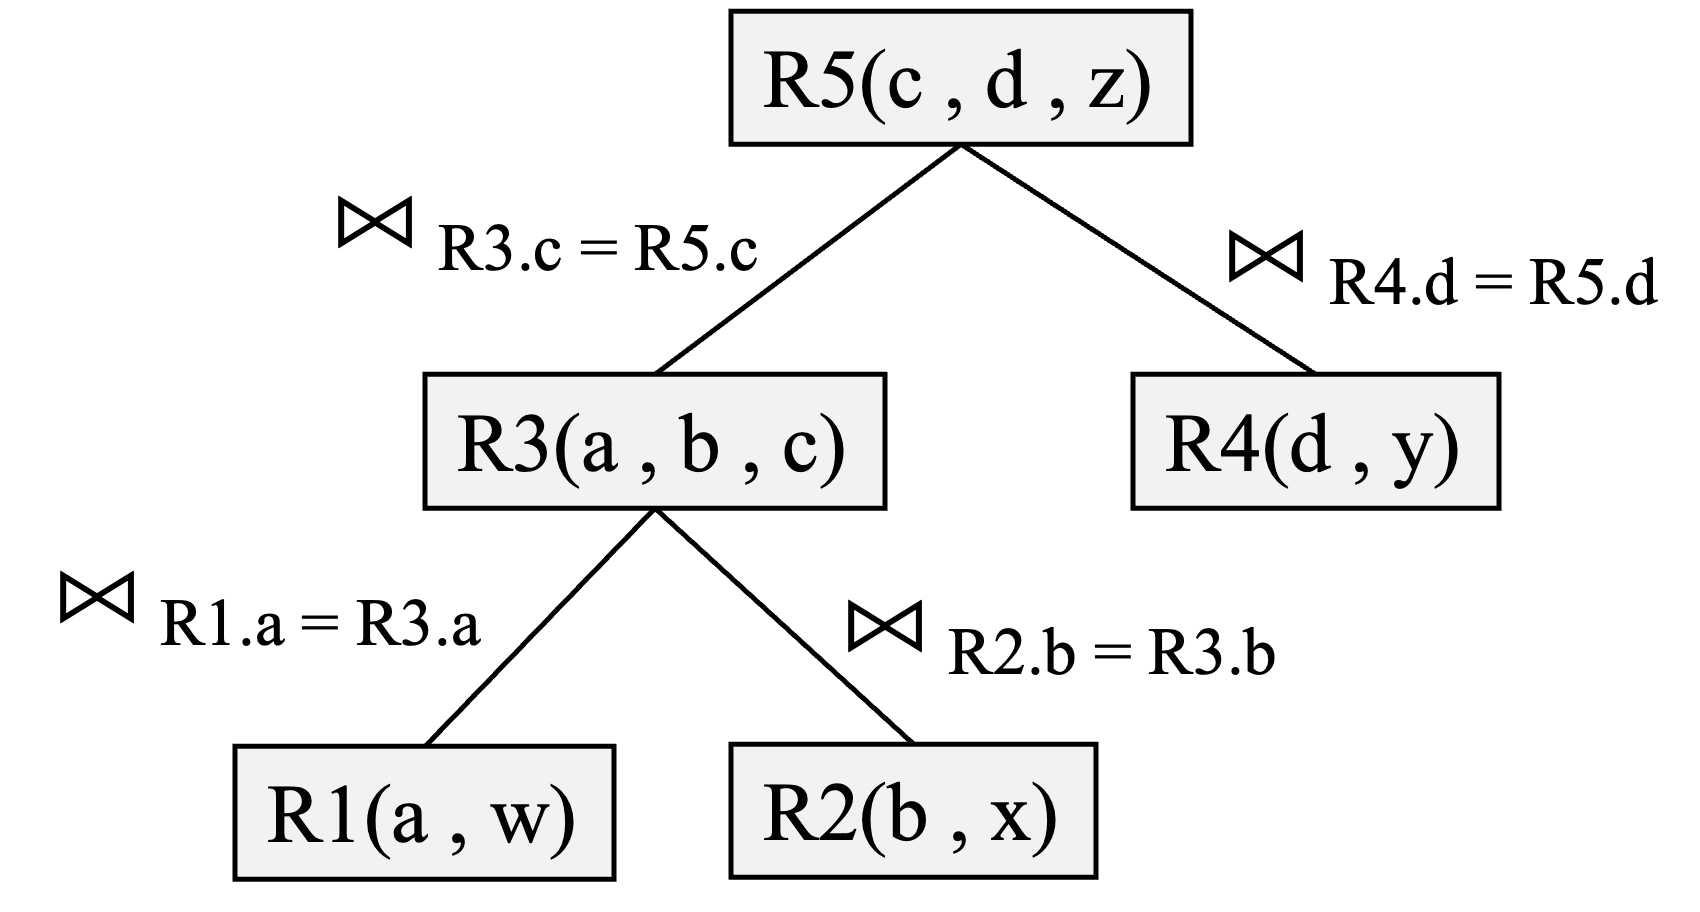
\includegraphics[width=0.5\linewidth]{figures/multi-way-join.png}
    \caption{A multi-way join tree of relations $R_1$ to $R_5$.}
    \label{fig:multiway-join}
\end{figure}

\system builds on the oblivious multi-way join algorithm of Wei and
Kerschbaum~\cite{ruidi2025oblivious}, referred to as \wei. Given $k$
relations $R_1, \ldots, R_k$ whose join predicates form an acyclic join
graph, \wei evaluates $R_1 \bowtie \cdots \bowtie R_k$ by constructing a
join tree (Figure~\ref{fig:multiway-join}). Concretely, \wei's access
pattern depends only on the sizes of the input relations and the final
join output size --- no intermediate result size is ever revealed.

The key abstraction is \emph{multiplicity}: rather than materializing
intermediate join results, \wei computes for every tuple $t$ a single
integer $\alpha_{\mathit{final}}(t)$: the number of rows in the final
result in which $t$ participates. Once these are known, it produces
the final output by replicating each tuple $\alpha_{\mathit{final}}(t)$
times and aligns the copies. The entire difficulty reduces to computing
multiplicities obliviously.

\Wei does this in two phases over the join tree. In the \textbf{bottom-up}
phase, each tuple is first assigned a \emph{local multiplicity}
$\alpha_{\mathit{local}}$: the number of partial results it participates
in within the subtree rooted at its relation. Leaf tuples start at
$\alpha_{\mathit{local}} = 1$. For each parent-child pair, it concatenates
the two relations and obliviously sorts them on the join attribute,
grouping tuples with matching keys. A linear scan aggregates, for each
parent tuple, the sum of local multiplicities of all matching child
tuples; the parent's local multiplicity is the product of contributions
across all its children. At the root, $\alpha_{\mathit{local}}$
equals $\alpha_{\mathit{final}}$ directly, since the root's subtree
is the entire tree.

The \textbf{top-down} phase propagates $\alpha_{\mathit{final}}$ from
the root downward using the same concatenate-sort-scan machinery in
reverse, combining each tuple's local multiplicity with the contribution
from outside its subtree. With all final multiplicities known, \wei
materializes the output in three steps: \emph{(i) expansion}, replicating
each tuple $\alpha_{\mathit{final}}$ times; \emph{(ii) alignment},
ordering matching tuples consistently across relations; and \emph{(iii)
merge}, combining aligned tuples into the final result.


The overall complexity is $O(N \log N + \mathit{OUT})$, where $N$ is the total 
input size and $\mathit{OUT}$ is the output size. \sujaya{@Bishwajit: Shouldn't there be a sort on the output size??} The dominant concrete cost is 
oblivious sorting: each parent-child pair requires six sorts, three per 
phase. \system reduces this cost by decomposing multi-hop queries to minimize 
join tree depth, as described in Section~\ref{sec:onehop}.
\section{Overview}
\label{sec:overview}

This section presents the intuition behind \system's approach through a 
running example from financial fraud detection.

\noindent\textit{Query.} Detect rapid 3-hop transfers of large amounts where 
money starts or ends in a newly opened account and moves across different 
owners.

\begin{verbatim}
MATCH (a1:Account)-[t1:TXN]->(a2:Account)
  -[t2:TXN]->(a3:Account)-[t3:TXN]->(a4:Account)
WHERE t1.amount > 10000
  AND t2.amount > 10000
  AND t3.amount > 10000
  AND t2.ts <= t1.ts + duration({minutes: 10})
  AND t3.ts <= t2.ts + duration({minutes: 10})
  AND ( a1.open_date >= date() - duration({days: 30})
    OR a4.open_date >= date() - duration({days: 30}))
  AND a1.owner_id <> a2.owner_id
  AND a2.owner_id <> a3.owner_id
  AND a3.owner_id <> a4.owner_id
RETURN a1.acc_id, a2.acc_id, a3.acc_id, a4.acc_id
\end{verbatim}

\noindent\textbf{Graph structure as an opportunity.} This query has a 
natural structure that a general-purpose join engine cannot see: every hop 
follows the same $n_i \rightarrow e \rightarrow n_j$ pattern, predicates 
are attached to specific nodes and edges rather than applied globally, and 
production graph databases maintain both forward and reverse edge lists.
These properties 
create an opportunity. For a single hop $n_i \rightarrow e \rightarrow n_j$, 
we evaluate the traversal from \emph{both ends simultaneously} --- 
probing forward edges from $n_i$ and reverse edges from $n_j$ in parallel 
--- and merge the results. Because edge table sizes are public in our threat 
model, the output is bound to $|E|$, revealing 
nothing beyond what is already known. We also fuse predicate filtering 
on $n_i$, $n_j$ and/or $e$ to the \onehop operator, so the unfiltered intermediate 
is \emph{never materialized} and its size is \emph{never revealed}. The 
entire one-hop traversal requires a single oblivious sort.

\noindent\textbf{Exploiting parallelism across hops.} A multi-hop query 
chains several such one-hop patterns. Crucially, patterns at different parts of the 
query are often \emph{independent}. \system proposes a query decomposer that
identifies these independent one-hop patterns and schedules them in 
parallel, as illustrated in Figure~\ref{fig:intuition}. For the 3-hop 
query above, the decomposer extracts one-hop patterns $H_1$ 
(over $a_1, t_1, a_2$) and $H_2$ (over $a_3, t_3, a_4$) and evaluates 
them simultaneously. Their outputs --- each of publicly known size $|E|$ 
--- feed into a residual join over $\{H_1, t_2, H_2\}$, which is handled
by \wei.

\begin{figure}
    \centering
    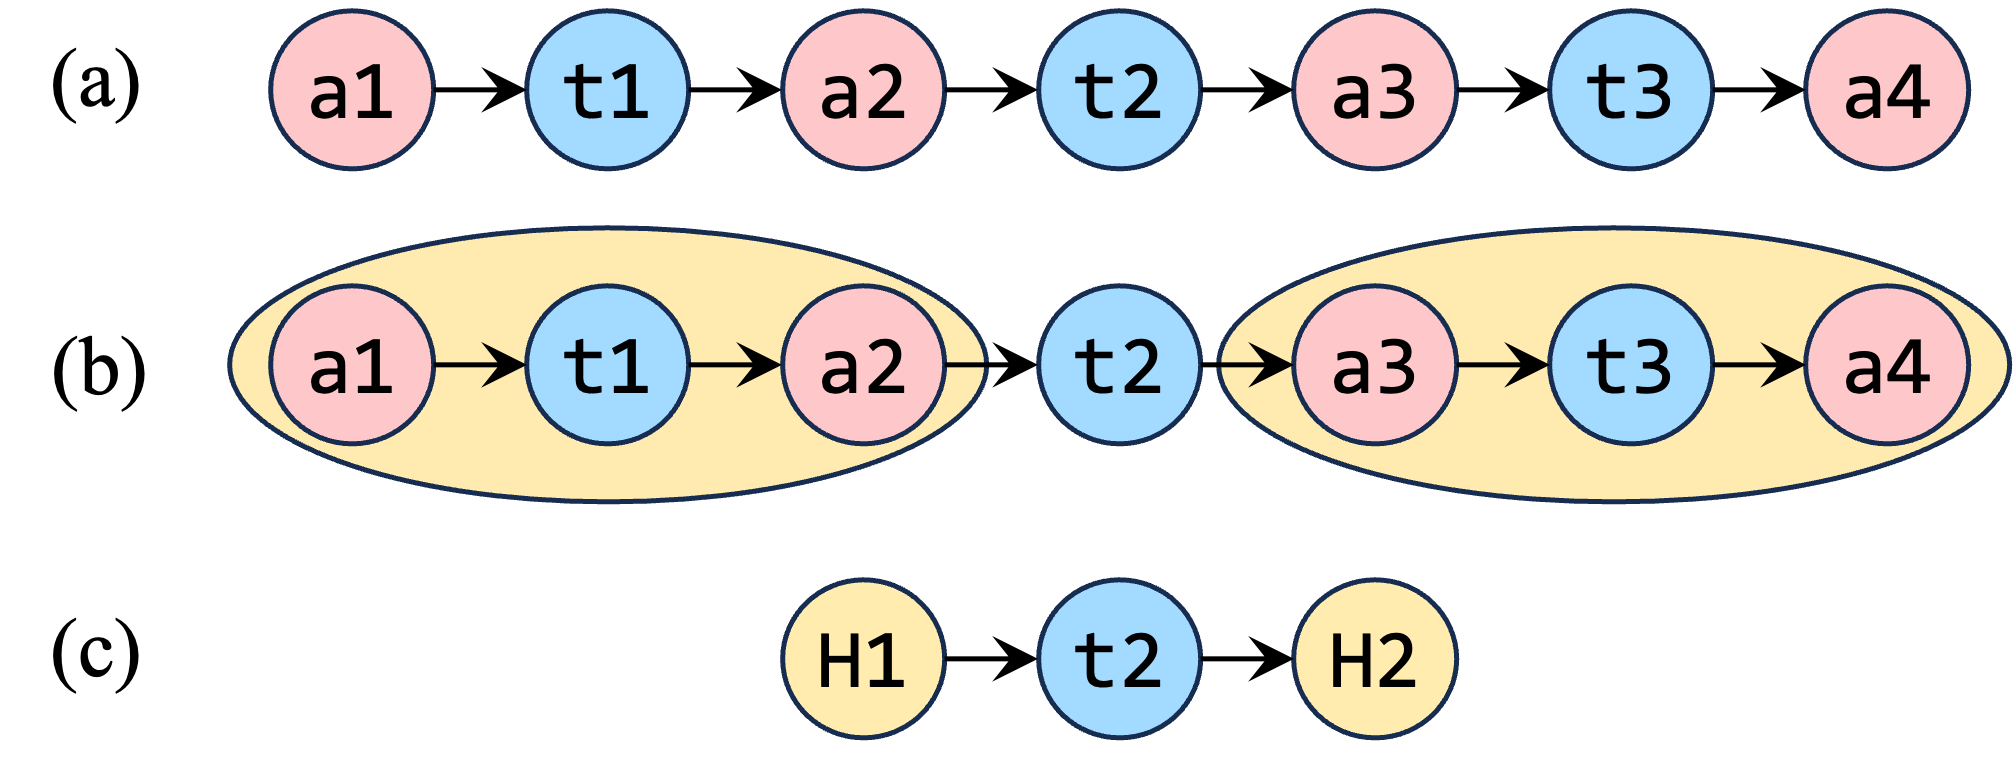
\includegraphics[width=0.7\linewidth]{figures/intuition-example.png}
    \caption{Decomposing a 3-hop query into parallel one-hop operators 
    ($H_1$, $H_2$) and a residual 3-way join, reducing a 7-way join tree 
    to a 3-way join tree.}
    \label{fig:intuition}
\end{figure}

\noindent\textbf{Why this outperforms applying \wei directly.}
Treating the query as a flat 7-way join and feeding it to \wei is 
correct but wasteful. Their scheme fails to
exploit bidirectional edges, cannot fuse predicates into the traversal, 
and processes the full join tree sequentially --- each parent-child pair 
in the tree requires six oblivious sorts (a total of XX for the 7-way join).
Worse, when predicates are present, \wei 
applies filtering only after the join materializes its output, exposing the 
unfiltered intermediate size to the adversary. \system avoids all of this: 
the one-hop operator collapses a three-way join into a single sort, the 
decomposer eliminates join depth by running independent hops in parallel, 
and in-place filtering ensures the adversary learns only the base table 
sizes, the query structure, and the final filtered result size.

\system's query processing engine comprises two components beyond \wei: 
the \onehop operator (Section~\ref{sec:onehop}), which implements the 
efficient single-sort traversal with in-place filtering, and the query 
decomposer (Section~\ref{sec:decomposition}), which identifies independent 
one-hop patterns and rewrites multi-hop queries into parallelizable 
components feeding a reduced residual join.
%==============================================================================
\section{The \Onehop Operator}
\label{sec:onehop}
%==============================================================================


This section presents the \onehop operator that computes the output for a 
single-hop pattern $n_i \rightarrow e \rightarrow n_j$ within an acyclic 
graph query. Specifically, given a source node $n_i(id, [prop])$ and destination 
node $n_j(id, [prop])$ connected by edge label $e$, each with its properties, 
the \onehop operator returns all tuples $(n_i, e, n_j)$, whose output size is 
bounded by $|e|$. The two nodes may be of the same or different types.
Additionally, \onehop marks output tuples that satisfy the query predicates 
$p_s$, $p_e$, and/or $p_d$ with a flag, leaving non-matching tuples unmarked. 
This flagging mechanism is central to hiding intermediate result sizes, as we 
describe in []. The \onehop operator reveals no information 
beyond the sizes of the source node table, destination node table, and the 
edge list --- all of which are public in our threat model.


Recall that similar to plaintext \gdbs~\cite{janusgraph, feng2023kuzu, 
deutsch2019tigergraph, sun2015sqlgraph}, \system also stores two versions of each 
edge list but without revealing the graph structure: a \textit{forward list} 
$E_F$ sorted by source node ids and a \textit{reverse list} $E_R$ sorted by 
destination node ids, both of size $|e|$.
The \onehop operator exploits both lists to parallelize one-hop query 
processing. We first describe a plaintext algorithm and then identify its 
leakages, which motivate our oblivious design.


\noindent\textbf{Plaintext algorithm.}
A natural plaintext approach proceeds as follows. Inspired by hash joins, 
store source node entries in a hash table and probe it once per entry in 
$E_F$, attaching matching source properties to each edge; the destination side
is handled symmetrically against $E_R$ in parallel. Then, sort one of the lists,
say $E_R$ on source ids, and merge the two lists row-wise, combining source node,
edge, and destination node properties into the output tuple. Finally, apply 
predicate filters on the source, destination, and edge properties, retaining 
only tuples that pass. This enables bidirectional parallel processing of the 
traversal.

\noindent\textbf{Leakages.}
The plaintext algorithm above has three sources of leakage that make it 
non-oblivious:
\begin{enumerate}[leftmargin=*]
    \item \textit{Hash table access pattern.} Hash table construction and probing
    reveals for each probe whether a match occurred and, if so, at which location,
    exposing which node ids appear in the edge list.

    \item \textit{Node degree.} A node id appears in the edge list once per 
    incident edge, so high-degree nodes are probed repeatedly. The number 
    of repeated probes to the same id reveals the degree distribution and 
    thus the graph structure.

    \item \textit{Predicate selectivity.} Filtering the merged output on 
    node and edge predicates reveals how many tuples satisfy predicates, 
    leaking the selectivity of query predicate values.
\end{enumerate}

We design the \onehop operator to retain the bidirectional parallelism of 
the plaintext algorithm while provably eliminating all three leakages.


% This
% creates two problems. First, the oblivious hash table we build [refer this] on permits each
% key to be queried \emph{at most once}, so repeated probes for the same source
% would violate its security precondition. Second, even setting that aside, the
% number of probes for a given id would equal that id's degree, directly exposing
% the graph's degree distribution. The operator resolves both by probing each
% distinct key \emph{exactly once} and then obliviously propagating the retrieved
% attributes to the remaining edges that share that key, so the access pattern
% depends only on $|E|$ --- never on any node's degree.


% An oblivious \onehop must hide three sources of leakage. First,
% \emph{hash-bucket access}: the memory pattern of retrieving a node's attributes
% by id would expose which key was probed. Second, \emph{node degree}: as pointed above, the number
% of source-side (or destination-side) lookups for a given id would equal its
% degree, leaking the degree distribution of the graph. Third, \emph{predicate
% selectivity}: the number of edges that satisfy the query predicates would reveal
% how many tuples match. The algorithm below neutralizes the first two by
% construction; the third is handled by always emitting $|E|$ rows and deferring
% any selectivity-dependent sizing, as we discuss at the end of the section.

%------------------------------------------------------------------------------
\subsection{\Onehop Algorithm}
\label{sec:onehop:algorithm}


We address the three leakages in order and present the operator in Algorithm~\ref{alg:onehop}.

\noindent\textbf{Addressing leakage 1: Hash table access pattern.}
Our algorithm stores source and destination node information in oblivious 
hash tables (\ohts). Our implementation utilizes H2O2RAM~\cite{zheng2025h2o2ram}
but the operator can use any \oht.
\ohts ensure that both table construction and probing are oblivious: the 
access pattern depends only on the input size, not on the values stored, and 
probing reveals neither whether a match was found nor the location of any 
matched entry. Note that \oht construction requires unique input keys, which is satisfied 
here since node ids used as keys for both source and destination tables
are unique by definition. However, \ohts do not protect against \emph{repeated probes 
of the same key} --- if the same node id is probed multiple times due to its 
degree in the edge list, that repetition remains visible. Node degree leakage 
therefore persists and is addressed next. 

\noindent\textit{Offline/online separation.}
\oht construction is generally expensive. For example, H2O2RAM's build complexity 
ranges from $O(n\log^2 n)$ for small tables to 
$O(n\log^2\log n)$ for large ones~\cite{zheng2025h2o2ram}. We observe, 
however, that in our operator the hash table acts as a \emph{index}
built on node entries and then probed by edge entries at query time. 
This means index construction can occur \emph{offline}, before any query 
arrives. Furthermore, once an index is built for nodes $n_i$ and $n_j$ 
paired with edge label $e$, it can be reused across all queries over the 
same node-edge combination, amortizing the construction cost. Note that 
the same \oht cannot be reused across different edge labels without 
reconstruction, so one index is required per $(n, e)$ pair. Changes to
a node or an edge also requires a reconstruction.




\begin{algorithm*}[t]
\caption{Oblivious \onehop Operator}
\label{alg:onehop}
\begin{algorithmic}[1]
\Require Forward list $E_{\!f}$ (sorted by $src\_id$), reverse list $E_{\!r}$
         (sorted by $dst\_id$); precomputed indices $H_S$, $H_D$; optional
         predicates $P$
\Ensure  Result $R$ with $|R| = |E|$
\Statex
\State \textbf{Source branch} \Comment{concurrent with the destination branch}
\State $\textsc{Dedup}(E_{\!f})$: for each row $i$,\algoIndent{1}
       $E_{\!f}[i].k \gets \textsc{OCmpSet}\big(E_{\!f}[i].src\_id = E_{\!f}[i\!-\!1].src\_id,\ \bot,\ E_{\!f}[i].src\_id\big)$
\State for each row $i$: probe $H_S[E_{\!f}[i].k]$ \Comment{all $|E|$ rows; dummy keys are no-ops}
\State $\textsc{Redup}(E_{\!f})$: for each row $i$,\algoIndent{1}
       $E_{\!f}[i].sattr \gets \textsc{OCmpSet}\big(E_{\!f}[i].k = \bot,\ E_{\!f}[i\!-\!1].sattr,\ E_{\!f}[i].sattr\big)$
\State $\textsc{Merge}(E_{\!f}, \text{source attributes})$ \Comment{attach source columns}
\Statex
\State \textbf{Destination branch} \Comment{symmetric over $dst\_id$, $H_D$}
\State $\textsc{Dedup}$ / probe $H_D$ / $\textsc{Redup}$ / $\textsc{Merge}$ on $E_{\!r}$
\State $E_{\!r} \gets \textsc{OSort}(E_{\!r})$ into edge order \Comment{re-align to source branch}
\Statex
\State \textbf{Combine}
\State $R \gets \textsc{Merge}(E_{\!f}, E_{\!r})$ \Comment{column-wise, aligned per edge}
\If{$P \neq \emptyset$} \Comment{standalone query only; skipped under decomposition}
    \State $R \gets \textsc{OCompact}\big(\text{rows of } R \text{ satisfying } P\big)$
\EndIf
\State \Return $R$
\end{algorithmic}
\end{algorithm*}

\noindent\textbf{Addressing leakage 2: Node degree.}
Since \ohts cannot protect against repeated probes to the same node id, the 
\onehop operator addresses node degree leakage as the first step of online 
processing. The key idea is to \emph{deduplicate} $E_F$ (and $E_R$ in 
parallel), replacing all but the first occurrence of each node id with a 
dummy, so that each distinct node id is probed exactly once.

Deduplication exploits the fact that $E_F$ is already sorted by source id 
and $E_R$ by destination id. A linear scan over each list compares each 
entry with its predecessor and replaces repeated ids with dummies using 
\cmpset, leaving the first occurrence of each distinct id as the only real
entry per run.

We then probe the hash table index \emph{once per row}, including dummies.
A dummy key 
resolves to a no-op that the table absorbs, while a real key retrieves its 
node attributes and appends them to the edge attributes. Probing every row, 
rather than only real ones, fixes the 
total probe count at $|E|$ regardless of the degree distribution, necessary
for maintaining obliviousness. 
\emph{Reduplication} then restores suppressed rows. Specifically,
a second linear scan 
propagates, via \cmpset, the retrieved attributes from each real row forward 
into all subsequent dummy rows in the same run, so every edge row ends up 
annotated with its source (or destination) node attributes. 

The source-side branch produces an annotated edge list ordered by $src\_id$, 
while the destination-side branch produces one ordered by $dst\_id$. To 
align them for merging, we obliviously sort the destination list by $src\_id$. 
A final \textsc{Merge} then combines the two lists row-wise, attaching both 
source and destination node attributes to each edge entry. This single 
re-alignment sort is the only oblivious sort in the entire \onehop operator.

\noindent\textbf{Addressing leakage 3: Predicate selectivity.}
To hide predicate selectivity, the operator linearly scans the merged list 
and annotates each row with a boolean flag indicating whether it satisfies 
the query predicates. What happens next depends on the operator's role in 
the query:

\begin{itemize}[leftmargin=*]
    \item {Standalone query.} The algorithm obliviously compacts the 
    flagged list and returns the result to the user. The output size equals 
    the final query result size, which is public under our threat model.

    \item {Component of a larger query.} Compaction is \emph{not} 
    performed. The output remains exactly $|E|$ rows, keeping intermediate sizes 
    independent of predicate 
    selectivity. The boolean flags are preserved for the downstream 
    multi-way join, which uses them to hide the final output size, as 
    discussed in [].
\end{itemize}

In both cases, the adversary learns nothing about how many rows satisfy the 
predicates until the final result size is deliberately released. \hfill$\Box$



% \paragraph{Two branches over the pre-sorted lists.}
% Because the forward and reverse edge lists are already maintained in sorted order
% (\Cref{sec:background:graph}), the operator needs no online sort to group edges by
% key --- the grouping comes for free from the storage layout. The source branch
% consumes the forward list and the destination branch the reverse list, and the
% two run concurrently on independent working copies.

% \paragraph{Deduplicate, probe, reduplicate.}
% Within a branch, \emph{deduplication} enforces the single-query-per-key
% constraint: in a linear scan over the sorted list, we compare each row's key with
% its predecessor and, using \textsc{OCmpSet}, obliviously replace it with a dummy
% ($\bot$) whenever the two match. Exactly one row per distinct key, the first in
% its run, keeps a live key. We then probe the index \emph{once for every row},
% dummies included; a dummy key resolves to a no-op the table absorbs, while live
% keys retrieve their node attributes. Probing every row, rather than only the live
% ones, keeps the query count equal to $|E|$ regardless of the graph's degree
% distribution; probing only live keys would let the query count leak the number of
% distinct sources. \emph{Reduplication} then refills the suppressed rows: a second
% scan copies, via \textsc{OCmpSet}, the probed attributes from the preceding row
% whenever the current key is a dummy, propagating each run's attributes forward. A
% \textsc{Merge} attaches the retrieved node attributes to the edge rows as new
% columns.

% \paragraph{Align and combine.}
% The source branch finishes in $src\_id$ order, but the destination branch finishes
% in $dst\_id$ order; we therefore oblivious-sort the destination branch back into
% the same per-edge order so the two $|E|$-row tables align row-for-row. A final
% \textsc{Merge} then combines them column-wise, giving every edge both its source
% and destination attributes. This single re-alignment is the operator's only online
% sort.

% \paragraph{Filtering.}
% When the operator answers a standalone one-hop query, we evaluate the predicates
% $P$ over every row after the combine and obliviously compact the matches; the
% result size is the query's (public) output size. When the operator instead serves
% as a building block under query decomposition (\Cref{sec:decomposition}), no
% predicates are applied here, and hence, the output remains exactly $|E|$ rows, keeping
% intermediate sizes independent of selectivity.

%------------------------------------------------------------------------------
% Alternatives considered (closes the section).
%------------------------------------------------------------------------------
The one-hop pattern could in principle be evaluated as two sequential 
oblivious binary joins using an operator such as 
Obliviator~\cite{mavrogiannakis2025obliviator}, at equal security but with 
two full join executions and an intermediate materialization. Our operator 
replaces this with one pass of probes per side and a single re-alignment 
sort, yielding a $1.1$--$1.7\times$ latency improvement over the two-join 
baseline (\Cref{sec:evaluation}).


%==============================================================================
\section{Query Decomposition}
\label{sec:decomposition}
%==============================================================================

The \onehop operator of \Cref{sec:onehop} evaluates a single edge pattern
$n_i \rightarrow e \rightarrow n_j$ obliviously, producing a hop relation
$h_e$
of publicly known size $|E_e|$ in a single oblivious sort. A $k$-edge
graph query chains $k$ such patterns together. Rather than treating the
full query as a monolithic join, we observe that it has two properties a
we can exploit.

\emph{Repeated structure.} Every edge in the query is a node-edge-node
traversal --- the exact pattern \onehop is optimized for. Evaluating the full
query as a single join discards this structure entirely, treating edge and
node tables as interchangeable relations.

\emph{Independent structure.} The hop over the first edge does not depend
on the result of the hop over the last edge. Hops at different parts of the
query can be evaluated simultaneously, with results combined only at the
end.

These two observations motivate \emph{query decomposition}: map every edge
in the pattern to a \onehop evaluation, run independent hops in parallel,
and combine the resulting hop-relations into a final answer. The
combination step requires joining $k$ hop-relations on their shared node
ids, where each of $k$ relations have publicly known
sizes. This is precisely what \wei is designed for: it evaluates acyclic
joins obliviously while hiding all intermediate result sizes. The 
query decomposer's goal is to
utilize \onehop wherever possible to efficiently handle the graph traversal
structure and \wei for the residual combination.

We illustrate each step of the decomposition on a running example: a
graph query over a social graph in which person $p_1$ knows
person $p_2$; $p_2$ created comment $c$ that carries tag $t$; and $p_2$
lives in city $\mathit{ci}$, with predicates pinning $p_1$, $t$, and
$\mathit{ci}$:
\begin{center}
\small\ttfamily
p1 -[knows]-> p2 -[created]-> c -[hasTag]-> t \\
\phantom{p1 -[knows]-> }p2 -[livesIn]-> ci \\
\upshape predicates:\ttfamily\ p1.id=933,\ t.id=7,\ ci.id=42
\end{center}
A \emph{query template} defines a node-edge traversal 
pattern and which properties 
are filtered but leaves the predicate values unspecified. A \textit{query},
issued at runtime, instantiates a template with concrete 
predicate values. In the running example, the query template has five 
node labels and four edge labels. We trace the decomposition through 
this example at each step below.

%------------------------------------------------------------------------------
\subsection{Query Templates and Hops}
\label{sec:decomposition:model}
%------------------------------------------------------------------------------

We model a graph query template as a directed \emph{pattern graph} $G_Q = (N,
\mathcal{E})$. Each node $n \in N$ has a label drawn from the schema 
(Section~\ref{sec:background:graph}), and each directed edge 
$e \in \mathcal{E}$ is identified by the triple $(S_e, E_e, D_e)$ --- 
the label of its source node, the edge label, and the label of its 
destination node. A query
also carries a set $P$ of predicates on node or edge properties.

A \emph{hop} $h_e$ is the \onehop evaluation of edge $e$ over its triple
$(S_e, E_e, D_e)$. It has exactly $|E_e|$ rows and carries the edge
attributes of $E_e$ together with the source- and destination-node
attributes, disambiguated by role: in $h_e$, a column is written as
$\mathit{label}\_\texttt{src}\_\mathit{col}$ or
$\mathit{label}\_\texttt{dst}\_\mathit{col}$. This naming lets two hops
that meet at a shared pattern node be joined unambiguously, where the shared node
appears as the destination of one hop and the source of the next, and the
column names make the equality explicit.

\noindent\textbf{Running example.} Each of the four edges becomes one hop:
\begin{center}
\small
\begin{tabular}{@{}ll@{}}
$h_1$: & \texttt{(p1:Person)-[knows]->(p2:Person)} \\
$h_2$: & \texttt{(p2:Person)-[created]->(c:Comment)} \\
$h_3$: & \texttt{(p2:Person)-[livesIn]->(ci:City)} \\
$h_4$: & \texttt{(c:Comment)-[hasTag]->(t:Tag)} \\
\end{tabular}
\end{center}
Note that $h_1$, $h_2$, and $h_3$
are independent of one another --- none consumes another's output --- and
can be evaluated in parallel. Each \onehop reads
only the base node or edge tables and not the output of any other hop.

%------------------------------------------------------------------------------
\subsection{The Decomposition Algorithm}
\label{sec:decomposition:algorithm}
%------------------------------------------------------------------------------

\Cref{alg:decompose} formalizes the procedure in three steps:
(\emph{i})~identify entry nodes and emit one hop per edge via BFS;
(\emph{ii})~stitch hops together on shared nodes; and
(\emph{iii})~place predicates on the appropriate hops. We describe each
step in turn.

\begin{algorithm*}[t]
\caption{Pattern Decomposition}
\label{alg:decompose}
\begin{algorithmic}[1]
\Require query graph $G_Q=(N,\mathcal{E})$ with label-typed nodes and
         directed edges $e=(\mathit{src}(e)\!\rightarrow\!\mathit{dst}(e))$
         typed $(S_e,E_e,D_e)$; node predicates $P$
\Ensure  Hop list $\mathcal{H}$ and reduced query $Q'$
\Statex
\State $\mathit{Roots} \gets \{\, n \in N : n=\mathit{src}(e)\text{ for
       some }e \text{ and } n\neq\mathit{dst}(e)\ \text{for all } e \,\}$
\State $\mathcal{H} \gets [\,]$;\quad $\mathit{seen} \gets \emptyset$
\For{each $r \in \mathit{Roots}$ in fixed order}
  \State $F \gets [\,r\,]$
  \While{$F \neq [\,]$}
    \State $u \gets \textsc{Pop}(F)$
    \For{each out-edge $e=(u\!\rightarrow\!w)$ with $e \notin
         \mathit{seen}$, in fixed order}
      \State $\mathit{seen} \gets \mathit{seen}\cup\{e\}$
      \State append hop $h_e=\langle S_e, E_e, D_e\rangle$ to $\mathcal{H}$
      \State $\textsc{Push}(F, w)$
    \EndFor
  \EndWhile
\EndFor
\Statex
\State $\mathcal{J} \gets \emptyset$
\For{each pattern node $n$ appearing in $\geq 2$ hops}
  \State let $h_{1},\dots,h_{m}$ be those hops in hop order, and
         $\rho_j\in\{\texttt{src},\texttt{dst}\}$ the role of $n$ in $h_j$
  \For{$j=1$ to $m-1$}
    \State $\mathcal{J} \gets \mathcal{J} \cup
           \{\, h_j.(\rho_j\text{-}\mathit{id}) =
           h_{j+1}.(\rho_{j+1}\text{-}\mathit{id}) \,\}$
  \EndFor
\EndFor
\Statex
\For{each predicate $p \in P$ on node $n$}
  \State $h \gets$ first hop in $\mathcal{H}$ with
         $n\in\{\mathit{src}(h),\mathit{dst}(h)\}$
  \State rewrite $p$'s column to $\mathit{label}\_\rho\_\mathit{col}$
         for $n$'s role $\rho$ in $h$
\EndFor
\State $Q' \gets$ join over $\{h\in\mathcal{H}\}$ with conditions
       $\mathcal{J}$ and the placed predicates
\State \Return $\mathcal{H},\ Q'$
\end{algorithmic}
\end{algorithm*}

\emph{Step 1: Entry nodes and hop emission.}
The traversal starts from \emph{entry nodes}: nodes in the query that are 
the source of some edge but the destination of none. A template may
have several entry nodes when it contains branches or disconnected
components; each seeds an independent BFS traversal. From each entry node,
BFS emits one hop per edge in a fixed order, visiting every out-edge of
each dequeued node. The decomposition is exhaustive: every edge becomes a
hop. Emitting hops uniformly keeps the rewrite a function of query
structure alone with no data-dependent choices, and hence no new leakage.

\noindent\textbf{Running example.} Node $p_1$ is the only entry node. BFS
visits $p_2$ next, which has two outgoing edges (\texttt{created} and
\texttt{livesIn}), emitting $h_2$ and $h_3$ in fixed order. From $c$, BFS
emits $h_4$. The four hops are produced in order $h_1, h_2, h_3, h_4$.

\emph{Step 2: Stitching hops.}
A shared node in the pattern graph --- one appearing in more than one hop --- must be
joined on its identity in the residual query. For each such node we collect
the hops in which it appears, note the role it plays in each (source or
destination), and add an id-equality between consecutive occurrences. Along
a chain the shared node is the destination of the earlier hop and the
source of the later, giving a $\mathit{dst}\text{-}\mathit{id} =
\mathit{src}\text{-}\mathit{id}$ condition. At a branch where the shared node is
the source of multiple hops, we get $\mathit{src}\text{-}\mathit{id} =
\mathit{src}\text{-}\mathit{id}$ conditions. Together these reconstruct
exactly the equalities of the original join.

\noindent\textbf{Running example.} Node $p_2$ is a branch: destination of
$h_1$, source of both $h_2$ and $h_3$. Node $c$ is shared between $h_2$
(destination) and $h_4$ (source). Stitching yields three join conditions:
\begin{center}
\small
\begin{tabular}{@{}ll@{}}
\texttt{h1.Person\_dst\_id = h2.Person\_src\_id} & (chain: $p_2$ in
$h_1{\to}h_2$)\\
\texttt{h2.Person\_src\_id = h3.Person\_src\_id} & (branch: $p_2$ in
$h_2, h_3$)\\
\texttt{h2.Comment\_dst\_id = h4.Comment\_src\_id} & (chain: $c$ in
$h_2{\to}h_4$)\\
\end{tabular}
\end{center}

\paragraph{Step 3: Placing predicates.}
Each node predicate is attached to the first hop containing its node and
rewritten against that hop's columns, qualified by the role the node plays
there. We evaluate predicates in \onehop whenever possible, which marks 
each row with a boolean indicating if it satisfied the predicates or not. However, as stated in \cref{sec:onehop}, the size of a \onehop operation
is always bound by its edge list size. 

\noindent\textbf{Running example.} Predicate $p_1.\mathit{id}=933$ lands
on $h_1$ (where $p_1$ is the source); $t.\mathit{id}=7$ lands on $h_4$
(where $t$ is the destination); $\mathit{ci}.\mathit{id}=42$ lands on
$h_3$ (where $\mathit{ci}$ is the destination). The complete residual
query handed to \wei is:
\begin{center}
\small
\begin{tabular}{@{}ll@{}}
$h_1 \bowtie h_2 \bowtie h_3 \bowtie h_4$ & \\[4pt]
\texttt{h1.Person\_dst\_id = h2.Person\_src\_id} & (chain: $p_2$ in $h_1{\to}h_2$)\\
\texttt{h2.Person\_src\_id = h3.Person\_src\_id} & (branch: $p_2$ in $h_2, h_3$)\\
\texttt{h2.Comment\_dst\_id = h4.Comment\_src\_id} & (chain: $c$ in $h_2{\to}h_4$)\\[4pt]
\texttt{h1.Person\_src\_id = 933} & (predicate on $p_1$)\\
\texttt{h4.Tag\_dst\_id = 7} & (predicate on $t$)\\
\texttt{h3.City\_dst\_id = 42} & (predicate on $\mathit{ci}$)\\
\end{tabular}
\end{center}
The residual
join over public-sized hop relations then evaluates them obliviously.
A nine-way join over five node labels and four edge labels becomes a
four-way join over four hop relations, each of publicly known size.

%------------------------------------------------------------------------------
\subsection{Parallelism and Comparison with Naive Execution}
\label{sec:decomposition:parallelism}
%------------------------------------------------------------------------------

To see the concrete benefit of query decomposition, consider a $k$-hop chain query evaluated two
ways. Applying \wei directly to the full $(2k{+}1)$-way join requires six
oblivious sorts per parent-child pair over a join tree of depth $2k$,
totaling $12k$ sorts. Moreover, each 
parent-child pair can only be evaluated in sequence in their scheme.
With decomposition, $k$ \onehop executions run in
parallel (one sort each), followed by \wei over the $k$-way residual join
(six sorts per pair over a tree of depth $k{-}1$, totaling $6(k{-}1)$
sequential sorts). The total is $k + 6(k{-}1) = 7k - 6$ sorts --- a reduction from
$12k$ to $7k{-}6$, with the $k$ \onehop sorts running in parallel rather
than sequentially. For $k=3$ this cuts sequential sort depth from 24 to 12,
and the parallel \onehop sorts contributes little to the critical path. The
gap widens with $k$. This enables our algorithm to handle input tables of XX M, whereas the baseline saturates at size YY.\sujaya{@Bish: please confirm these comparisons}

%------------------------------------------------------------------------------
\subsection{Correctness and Data Independence}
\label{sec:decomposition:correctness}
%------------------------------------------------------------------------------

\paragraph{Correctness.}
Each hop $h_e$ equals the three-way join $S_e \bowtie E_e \bowtie D_e$
(\Cref{sec:onehop}). The stitch conditions reintroduce precisely the
foreign-key equalities of the original pattern, and predicates are
reattached unchanged. The reduced query $Q'$ therefore computes the same
relation as the original $(2k{+}1)$-way join.

\paragraph{Data independence.}
Every choice the procedure makes --- entry nodes, traversal order, hop
emission, stitch conditions, and predicate placement --- is a function of
the query graph and predicate columns alone, both public under our threat
model (\Cref{sec:background:threat}). No data value is read. Each hop has
public size $|E_e|$, and feeding public-sized hops to \wei keeps every
intermediate size public. The composition leaks nothing beyond what the
inputs already reveal.

%------------------------------------------------------------------------------
\subsection{Homogeneous Graphs}
\label{sec:decomposition:homogeneous}
%------------------------------------------------------------------------------

When all edges share one triple --- as in the banking workload of
\Cref{sec:evaluation}, where every edge is typed
$(\texttt{Account})\text{-}[\texttt{Txn}]\text{-}(\texttt{Account})$ ---
all hops are instances of a single hop relation, and the residual query
degenerates to a self-join of that relation under the stitch and predicate
conditions. This homogeneous case requires no algorithmic change and can
benefit from computing the \onehop operator only once.


% \section{Query Decomposition}
% \label{sec:decomposition}
% %==============================================================================

% The \onehop operator of \Cref{sec:onehop} evaluates a single edge pattern
% $n_i \rightarrow e \rightarrow n_j$. A general graph query, however, connects
% $k$ edges into an acyclic join graph and therefore corresponds to a
% $(2k{+}1)$-way join over $k{+}1$ node labels and $k$ edge labels. Handing such a
% query in full to the oblivious multi-way join \wei (\Cref{sec:background:joins})
% discards exactly the structure \onehop was built to exploit: every edge in the
% pattern is itself a one-hop join whose result has the publicly known size $|E|$.

% \system therefore \emph{decomposes} the pattern. Each edge is evaluated by a
% \onehop into a \emph{hop relation} of public size; the residual query then joins
% these hop relations rather than the original node and edge labels. Because each
% hop relation already carries its endpoints' attributes, the residual join is
% narrower: one input per edge instead of $2k{+}1$ base labels. Crucially, the rewrite
% is a \emph{structural} transformation: it reads only the query --- labels, the
% edge connectivity, and the columns named by predicates --- and never inspects a
% single data value, so it introduces no new leakage.

% While \wei evaluates any acyclic join graph, the decomposition is more
% specialized. It assumes the node--edge--node shape of a graph traversal: each hop joins a source
% node, an edge, and a destination node, and the edge relation in the middle
% carries the foreign keys to both endpoints --- exactly the relation \onehop
% enriches from either side. A join with no such middle relation, such as a direct
% node-to-node join, has nothing to fill and falls outside the decomposition. In
% the graph setting this costs nothing: traversals are mediated by edges, so two
% nodes meet only through an edge table, never directly. Every graph pattern
% therefore already has the shape the decomposition assumes, and \wei remains the
% general engine behind it.

% %------------------------------------------------------------------------------
% \subsection{query graphs and Hops}
% \label{sec:decomposition:model}
% %------------------------------------------------------------------------------

% We model a pattern query as a directed \emph{query graph} $G_Q = (N,
% \mathcal{E})$. Each node $n \in N$ carries a label drawn from the schema, and
% each edge $e \in \mathcal{E}$ is directed from a source node $\mathit{src}(e)$ to
% a destination node $\mathit{dst}(e)$. An edge is \emph{typed} by the triple
% $(S_e, E_e, D_e)$ --- its source label, edge label, and destination label. A
% query also carries a set $P$ of predicates on node properties.

% A \emph{hop} $h$ is the \onehop evaluation of one edge $e$ over its triple
% $(S_e, E_e, D_e)$. Following \Cref{sec:onehop}, $h$ has exactly $|E_e|$ rows and
% schema consisting of the edge attributes of $E_e$ together with the source- and
% destination-node attributes, the latter disambiguated by the role in which the
% node appears. We write a hop column as $\mathit{label}\_\texttt{src}\_\mathit{col}$
% or $\mathit{label}\_\texttt{dst}\_\mathit{col}$, recording the node label, the
% role (source or destination), and the original property name. This naming is what
% lets two hops that meet at a shared pattern node be joined unambiguously: the same
% node is reached as the destination of one hop and the source of the next.

% Two facts about a hop are central to the rest of the section. First, a hop's size
% $|E_e|$ is public, so a hop relation can be fed to \wei without revealing any
% selectivity. Second, a hop is type-specific: hops for differently typed edges are
% distinct relations, while hops for identically typed edges share one relation.

% %------------------------------------------------------------------------------
% \subsection{The Decomposition Algorithm}
% \label{sec:decomposition:algorithm}
% %------------------------------------------------------------------------------

% \Cref{alg:decompose} states the procedure. It traverses the query graph,
% emits one hop per edge, reconnects the hops on their shared nodes, attaches the
% predicates, and returns a reduced query $Q'$ for \wei.

% \begin{algorithm*}[t]
% \caption{Pattern Decomposition}
% \label{alg:decompose}
% \begin{algorithmic}[1]
% \Require query graph $G_Q=(N,\mathcal{E})$ with label-typed nodes and directed
%          edges $e=(\mathit{src}(e)\!\rightarrow\!\mathit{dst}(e))$ typed
%          $(S_e,E_e,D_e)$; node predicates $P$
% \Ensure  Hop list $\mathcal{H}$ and reduced query $Q'$
% \Statex
% \State $\mathit{Roots} \gets \{\, n \in N : n=\mathit{src}(e)\text{ for some }e
%        \text{ and } n\neq\mathit{dst}(e)\ \text{for all } e \,\}$
% \State $\mathcal{H} \gets [\,]$;\quad $\mathit{seen} \gets \emptyset$
% \For{each $r \in \mathit{Roots}$ in fixed order} \Comment{BFS: one hop per edge}
%   \State $F \gets [\,r\,]$ \Comment{frontier queue}
%   \While{$F \neq [\,]$}
%     \State $u \gets \textsc{Pop}(F)$
%     \For{each out-edge $e=(u\!\rightarrow\!w)$ with $e \notin \mathit{seen}$, in fixed order}
%       \State $\mathit{seen} \gets \mathit{seen}\cup\{e\}$
%       \State append hop $h_e=\langle S_e, E_e, D_e\rangle$ to $\mathcal{H}$
%       \State $\textsc{Push}(F, w)$
%     \EndFor
%   \EndWhile
% \EndFor
% \Statex
% \State $\mathcal{J} \gets \emptyset$ \Comment{stitch: shared node $\Rightarrow$ id-equality}
% \For{each pattern node $n$ appearing in $\geq 2$ hops}
%   \State let $h_{1},\dots,h_{m}$ be those hops in hop order, and
%          $\rho_j\in\{\texttt{src},\texttt{dst}\}$ the role of $n$ in $h_{j}$
%   \For{$j=1$ to $m-1$}
%     \State $\mathcal{J} \gets \mathcal{J} \cup
%            \{\, h_{j}.(\rho_j\text{-}\mathit{id}) = h_{j+1}.(\rho_{j+1}\text{-}\mathit{id}) \,\}$
%   \EndFor
% \EndFor
% \Statex
% \For{each predicate $p \in P$ on a node $n$} \Comment{place on first hop holding $n$}
%   \State $h \gets$ first hop in $\mathcal{H}$ with $n\in\{\mathit{src},\mathit{dst}\}$
%   \State rewrite $p$'s column to $\mathit{label}\_\rho\_\mathit{col}$ for $n$'s role $\rho$ in $h$
% \EndFor
% \State $Q' \gets$ join over $\{h\in\mathcal{H}\}$ with conditions $\mathcal{J}$ and the placed predicates
% \State \Return $\mathcal{H},\ Q'$
% \end{algorithmic}
% \end{algorithm*}

% \paragraph{Entry nodes.}
% The traversal starts from the pattern's \emph{entry nodes}: those that are the
% source of some edge but the destination of none. These are the heads of the
% pattern, fixed entirely by its connectivity. A pattern may have several entry
% nodes (disconnected components or several in-bound-free starts); each seeds an
% independent traversal.

% \paragraph{One hop per edge.}
% From each entry node we perform a breadth-first traversal that emits one hop for
% every edge, in a fixed order. The decomposition is therefore \emph{exhaustive}:
% every edge of the pattern becomes a hop, with no cost-based selection among
% edges. This is deliberate. Each hop replaces a three-way slice of the join by a
% single $|E|$-sized relation, and emitting them uniformly keeps the rewrite --- and
% hence the access pattern of producing it --- a function of the query alone.

% \paragraph{Branches.}
% A node with more than one outgoing edge yields more than one hop sharing that
% node as their source; the traversal handles such branches with no special case,
% since it simply visits every out-edge of each dequeued node. Chains are the
% special case in which every node has at most one outgoing edge.

% \paragraph{Stitching hops.}
% Wherever two hops meet at the same pattern node, the reduced query must join them
% on that node's identity. We collect, for each node shared by several hops, the
% hops in which it appears together with its role in each, and chain consecutive
% occurrences by an id-equality. Along a path the shared node is the destination of
% the earlier hop and the source of the later one, giving a
% $\mathit{dst}\text{-}\mathit{id} = \mathit{src}\text{-}\mathit{id}$ condition; at a
% branch the node is the source of both hops, giving a
% $\mathit{src}\text{-}\mathit{id} = \mathit{src}\text{-}\mathit{id}$ condition.
% Together these reconstruct exactly the equalities of the original join.

% \paragraph{Placing predicates.}
% Each node predicate is attached to the first hop that contains its node and
% rewritten against that hop's columns, qualified by the role (source or
% destination) the node plays there. Predicates become selection conditions of the
% reduced query, evaluated by \wei rather than inside the operator: as noted in
% \Cref{sec:onehop}, keeping predicates out of the per-hop \onehop preserves its
% $|E|$-sized, selectivity-independent output, so no intermediate size depends on
% how many rows match.

% %------------------------------------------------------------------------------
% \subsection{Example}
% \label{sec:decomposition:example}
% %------------------------------------------------------------------------------

% Consider a heterogeneous pattern over a social graph: a person $p_1$ who knows
% $p_2$; $p_2$ authored a comment $c$ that carries tag $t$; and $p_2$ lives in city
% $\mathit{ci}$, with predicates pinning $p_1$, $t$, and $\mathit{ci}$:
% \begin{center}
% \small\ttfamily
% p1 -[knows]-> p2 -[created]-> c -[hasTag]-> t \\
% \phantom{p1 -[knows]-> }p2 -[livesIn]-> ci \\
% \upshape predicates:\ttfamily\ p1.id=933,\ t.id=7,\ ci.id=42
% \end{center}

% The only entry node is $p_1$ (every other node is some edge's destination). The
% breadth-first traversal emits four hops, each with a \emph{different} triple:
% \begin{center}
% \small
% \begin{tabular}{@{}l@{}}
% $h_1$: \texttt{(Person)-[knows]->(Person)}\\
% $h_2$: \texttt{(Person)-[created]->(Comment)}\\
% $h_3$: \texttt{(Person)-[livesIn]->(City)}\\
% $h_4$: \texttt{(Comment)-[hasTag]->(Tag)}\\
% \end{tabular}
% \end{center}
% Node $p_2$ is a branch: it is the destination of $h_1$ and the source of both
% $h_2$ and $h_3$. Stitching on the shared nodes ($p_2$ and $c$) and placing the
% three predicates on the first hop holding each node yields the reduced query:
% \begin{center}
% \small
% \begin{tabular}{@{}l@{}}
% \texttt{h1.Person\_dst\_id = h2.Person\_src\_id} \quad\textrm{(stitch $p_2$)}\\
% \texttt{h2.Person\_src\_id = h3.Person\_src\_id} \quad\textrm{(branch $p_2$)}\\
% \texttt{h2.Comment\_dst\_id = h4.Comment\_src\_id} \quad\textrm{(stitch $c$)}\\
% \texttt{h1.Person\_src\_id = 933}\\
% \texttt{h3.City\_dst\_id = 42}\\
% \texttt{h4.Tag\_dst\_id = 7}\\
% \end{tabular}
% \end{center}
% A nine-way join over five node labels and four edge labels becomes a four-way
% join over four typed hop relations, each of public size, which \wei evaluates.

% %------------------------------------------------------------------------------
% \subsection{Correctness and Data Independence}
% \label{sec:decomposition:correctness}
% %------------------------------------------------------------------------------

% \paragraph{Correctness.}
% Each hop equals the three-way join $S_e \bowtie E_e \bowtie D_e$ of its edge
% (\Cref{sec:onehop}). The stitch conditions reintroduce precisely the
% foreign-key equalities of the original pattern --- a shared pattern node induces
% the same id-equality whether expressed over base labels or over the hops that
% meet at it --- and the predicates are reattached unchanged. Hence the reduced
% query $Q'$ computes the same relation as the original $(2k{+}1)$-way join.

% \paragraph{Data independence.}
% Every choice the procedure makes --- the entry nodes, the traversal order, which
% edges become hops, the stitch conditions, and where predicates land --- is a
% function of the query graph and the predicate columns, all of which are public
% under our threat model (\Cref{sec:background:threat}). No data value is read.
% The decomposition is thus fixed once the query is fixed, and each hop it produces
% has the public size $|E_e|$; feeding hops of public size to \wei keeps every
% intermediate size public, so the composition leaks nothing beyond the inputs.
% %------------------------------------------------------------------------------
% \subsection{Homogeneous Graphs}
% \label{sec:decomposition:homogeneous}
% %------------------------------------------------------------------------------

% When a query ranges over a single node label and a single edge label --- as in
% the banking workload of \Cref{sec:evaluation}, where every edge is typed
% $(\texttt{Account})\text{-}[\texttt{Txn}]\text{-}(\texttt{Account})$ --- all hops
% share one triple and are therefore instances of a \emph{single} hop relation.
% The reduced query then degenerates to a self-join of that relation under the
% stitch and predicate conditions of \Cref{alg:decompose}. This homogeneous case
% requires no change to the algorithm; it is simply the point at which the typed
% hop relations of the general procedure coincide, and it is the configuration we
% evaluate in \Cref{sec:evaluation}.

% \paragraph{Parallelism.}
% The hops are independent of one another. Each is produced by a separate \onehop
% that reads only its own edge's tables and writes only its own $|E_e|$-sized
% relation; no hop consumes another's result. All hops of a query can therefore be
% computed in parallel, leaving only the residual join over them to run
% sequentially through \wei. Since the number of hops and their sizes are fixed by
% the query, this parallelism is itself data-independent and adds no leakage.

\section{Oblivious Multi-way Join with Filters}
\label{sec:bandjoin}

The residual query produced by \Cref{sec:decomposition} joins $k$ hop-relations
on their shared node ids and evaluates predicate filters on node
and edge properties. A natural extension of \wei to support filtered joins would treat
filtering as a post-processing step: materialize the full join output of
size $\mathit{OUT}_{\mathit{join}}$, then apply predicates to produce the
final result of size $\mathit{OUT}_{\mathit{filtered}}$. Schemes that
explicitly support filtering, such as
Obliviator~\cite{mavrogiannakis2025obliviator}, Opaque~\cite{zheng2017opaque}, and
ObliDB~\cite{eskandarian2019oblidb}, follow this
approach, revealing both sizes to the adversary and allocating memory
proportional to the unfiltered join output, \textit{which for selective
predicates can be orders of magnitude larger than the final result}.


\system avoids this by integrating filtering directly into the
multiplicity computation of \wei. Recall from
\Cref{sec:background:joins} that \wei associates every tuple with a final
multiplicity $\alpha_{\mathit{final}}$ --- the number of times it appears
in the output --- and that all downstream multiplicities are products. We
observe that a
tuple with $\alpha_{\mathit{final}} = 0$ also flows through every phase
identically to any other tuple: same memory accesses, same loop bounds,
same allocations. It simply expands to zero output rows in the expansion
phase, contributing nothing to the result.

\noindent\textbf{Filter as multiplicity.}
Each \onehop operator produces a hop relation of publicly known size $|E_e|$ in
which every row carries a boolean flag indicating whether that row passes
the query predicates (\Cref{sec:onehop}). When this hop relation enters
\wei as a leaf, we initialize its local multiplicity as:
\[
\alpha_{\mathit{local}}(t) =
\begin{cases}
1 & \text{if } t\text{'s filter flag is set,} \\
0 & \text{otherwise.}
\end{cases}
\]
Because all multiplicities propagate as products up and down the join
tree, a single $0$ at any tuple \textit{zeroes out its entire contribution to}
$\alpha_{\mathit{final}}$. A tuple that fails a filter never participates
in any output row, exactly as if it had been removed --- but it is never
actually removed, and no branch or allocation ever reflects its absence.
The adversary observes only $\mathit{OUT}_{\mathit{filtered}}$, the size
of the final filtered result, and never learns the size the join would
have produced without filtering.

\noindent\textbf{Correctness.} The modified initialization is the only
change to \wei's pipeline. All other phases --- bottom-up, top-down,
expansion, and alignment --- proceed identically. A tuple that fails a
filter has $\alpha_{\mathit{final}} = 0$ and expands to zero rows;
a tuple that passes has its multiplicity computed exactly as in the
unfiltered join. The output is therefore identical to first joining and
then filtering.

\noindent\textbf{Obliviousness.} Since $\alpha_{\mathit{local}}$ is
initialized from a flag stored inside the tuple rather than from any
branching on the tuple's value, the memory access pattern of every
phase remains a function of the input sizes and $\mathit{OUT}_{\mathit{filtered}}$
alone. No intermediate count
is allocated, computed, or revealed.

\noindent\textbf{Applicability.} The same technique applies to any
multiplicity-based oblivious join scheme. Obliviator~\cite{mavrogiannakis2025obliviator},
for instance, explicitly reveals both the join output size and the
filtered output size as separate public quantities. Replacing its
post-join filter with the multiplicity initialization above collapses
these two leakages into one, revealing only
$\mathit{OUT}_{\mathit{filtered}}$. The modification requires no
structural change to the underlying join algorithm.

% \section{The Oblivious Multi-Way Band Join, Step by Step}
% \label{sec:bandjoin}


% The residual query produced by the decomposition of \Cref{sec:decomposition} is
% evaluated by the oblivious multi-way join engine \wei
% (\Cref{sec:background:joins}). This section walks through that engine
% operationally, at the level of detail needed to follow the remainder of the
% paper. We first restate the one invariant the whole construction is built to
% preserve, then introduce the \emph{multiplicity} abstraction that drives it, and
% finally trace the four phases end to end on a small example. Throughout, we
% generalize from equality joins to \emph{band} joins, the form \system actually
% needs.

% %------------------------------------------------------------------------------
% \subsection{What ``oblivious'' must mean here}
% \label{sec:bandjoin:invariant}
% %------------------------------------------------------------------------------

% Under our threat model (\Cref{sec:background:threat}), the adversary observes the
% full sequence of memory accesses, the control flow, and the size of every
% allocation. The join is \emph{oblivious} when all of this observable behavior is
% a function of only three \emph{public} quantities:
% \begin{enumerate}[label=(\roman*),leftmargin=2.2em,itemsep=2pt]
%   \item the sizes of the input relations $|R_1|,\dots,|R_k|$;
%   \item the size of the output, $\mathit{OUT}$; and
%   \item the query itself --- its schema, predicates, and join tree.
% \end{enumerate}
% No branch, loop bound, array index, or buffer size may depend on a \emph{value}
% inside a tuple, nor on any intermediate count (such as how many tuples match a
% given key). The challenge the algorithm solves is to compute a join --- an
% inherently data-dependent operation --- while letting only these three public
% quantities show through. Every phase below meets this bar by replacing
% data-dependent control flow with two fixed-shape primitives: the \emph{oblivious
% sort} (osort), whose comparison network is fixed by the input length alone, and
% the \emph{linear scan}, a single left-to-right pass that applies the same
% branchless update to every adjacent pair of tuples.

% %------------------------------------------------------------------------------
% \subsection{The central abstraction: multiplicities}
% \label{sec:bandjoin:multiplicity}
% %------------------------------------------------------------------------------

% The engine never materializes an intermediate join. Instead it computes, for
% every input tuple $t$, a single integer: the number of rows of the \emph{final}
% result in which $t$ participates. We call this its final multiplicity
% $\alpha_{\mathit{final}}(t)$. Once these numbers are known, producing the output
% is mechanical --- copy each tuple $\alpha_{\mathit{final}}(t)$ times and line the
% copies up --- so the entire difficulty is reduced to computing multiplicities
% obliviously.

% Two facts make this abstraction powerful. First, $\alpha_{\mathit{final}}$
% factors along the join tree: a tuple's count in the whole join is its count
% within its own subtree times the count contributed by the rest of the tree.
% This is what lets the engine compute it in two sweeps --- one up the tree, one
% down. Second, because each output row contains exactly one tuple from each
% relation, the multiplicities of any single relation sum to $\mathit{OUT}$;
% summing $\alpha_{\mathit{final}}$ over a relation is how the engine learns the
% (public) output size without ever inspecting a value.

% \paragraph{Band predicates.}
% A child tuple $c$ matches a parent tuple $p$ not on equality but on a
% \emph{band}: $c.\mathit{key} \in [\,p.\mathit{key}+\delta_1,\ p.\mathit{key}+\delta_2\,]$,
% where $\delta_1,\delta_2$ are constants of the predicate (equality is the special
% case $\delta_1=\delta_2=0$, and one-sided inequalities use $\pm\infty$ bounds).
% The engine handles a band with a \emph{boundary} technique: for each parent
% tuple it emits two marker tuples, a \textsc{start} at $p.\mathit{key}+\delta_1$
% and an \textsc{end} at $p.\mathit{key}+\delta_2$. After an osort on the key,
% every child that matches $p$ falls between $p$'s two markers, so the number of
% matches is the difference of two running counts read off at the markers --- a
% quantity a single linear scan computes for all parents at once.

% %------------------------------------------------------------------------------
% \subsection{The four phases}
% \label{sec:bandjoin:phases}
% %------------------------------------------------------------------------------

% Given the join tree, the engine runs four phases in order. The first two compute
% multiplicities; the last two turn them into output. We describe each by its
% \emph{goal}, its \emph{mechanism}, and what it \emph{leaves behind}.

% \paragraph{Phase 1 --- Bottom-up: local multiplicities.}
% \emph{Goal.} Give every tuple $t$ its local multiplicity
% $\alpha_{\mathit{local}}(t)$: the number of partial results it participates in
% within the subtree rooted at its relation.
% \emph{Mechanism.} Every leaf tuple starts at $\alpha_{\mathit{local}}=1$. The
% engine then visits parent--child pairs in post-order. For each pair it
% concatenates the two relations (the parent expanded into \textsc{start}/\textsc{end}
% boundary tuples), osorts on the join key so matching children are bracketed by
% their parent's markers, and runs a linear scan that accumulates, for each parent
% tuple, the sum of its matching children's multiplicities. Multiplying in this
% contribution updates the parent's $\alpha_{\mathit{local}}$.
% \emph{Leaves behind.} After the sweep reaches the root, each tuple carries the
% size of the join of its own subtree. At the root specifically,
% $\alpha_{\mathit{local}}=\alpha_{\mathit{final}}$, since the root's subtree is the
% whole tree.

% \paragraph{Phase 2 --- Top-down: final multiplicities.}
% \emph{Goal.} Turn every tuple's local multiplicity into its final multiplicity
% $\alpha_{\mathit{final}}$ --- its count in the \emph{entire} join, not just its
% subtree.
% \emph{Mechanism.} Starting from the root (whose count is already final), the
% engine visits parent--child pairs in pre-order. Using the same
% concatenate--osort--scan machinery, but with the predicate read in the opposite
% direction, it pushes each parent's final count down to its children, distributing
% it across the matching children in proportion to their local multiplicities.
% \emph{Leaves behind.} Every tuple in every relation now carries
% $\alpha_{\mathit{final}}$, together with an offset that records where its copies
% belong in the output (used for alignment in Phase 4).

% \paragraph{Phase 3 --- Distribute-and-expand: replicate each tuple.}
% \emph{Goal.} Physically realize the counts: each relation must become a buffer in
% which tuple $t$ appears exactly $\alpha_{\mathit{final}}(t)$ times, padded to its
% output length.
% \emph{Mechanism.} A linear scan over a relation takes the prefix sum of
% $\alpha_{\mathit{final}}$, which gives both each tuple's destination offset and
% the relation's output size $\mathit{OUT}$. Tuples with count zero contribute
% nothing and are discarded; the survivors are scattered to their offsets by a
% fixed sequence of power-of-two ``distribute'' passes, leaving padding gaps
% between groups, and a final linear scan copies each tuple rightward to fill its
% gap. The number and stride of these passes depend only on $\mathit{OUT}$.
% \emph{Leaves behind.} Every relation in the tree now has exactly $\mathit{OUT}$
% rows, with each tuple occupying as many consecutive slots as its multiplicity.

% \paragraph{Phase 4 --- Align-and-merge: assemble the result.}
% \emph{Goal.} Glue the expanded relations together so that row $i$ holds a single,
% consistent combination of one tuple from each relation --- i.e.\ the $i$-th join
% result.
% \emph{Mechanism.} Walking the tree from the root, the engine osorts each child by
% an \emph{alignment key} derived from the offset recorded in Phase 2, so that the
% child's copies land in the same row order as the partial result they extend. It
% then concatenates the child's columns onto the accumulating result with a single
% lockstep pass over the two equal-length buffers.
% \emph{Leaves behind.} The accumulated relation at the root is the materialized
% join, of size $\mathit{OUT}$.

% %------------------------------------------------------------------------------
% \subsection{A worked example}
% \label{sec:bandjoin:example}
% %------------------------------------------------------------------------------

% Consider a two-relation equality join with parent $P=\{p_1,p_2\}$ and child
% $C=\{c_1,c_2,c_3\}$, where $p_1$ matches $c_1,c_2$ and $p_2$ matches $c_3$.

% \begin{itemize}[leftmargin=1.4em,itemsep=2pt]
%   \item \textbf{Phase 1.} Leaves $c_1,c_2,c_3$ start at
%         $\alpha_{\mathit{local}}=1$. The bottom-up scan over the $P$--$C$ pair
%         finds two matching children under $p_1$ and one under $p_2$, giving
%         $\alpha_{\mathit{local}}(p_1)=2$, $\alpha_{\mathit{local}}(p_2)=1$. As
%         root, these are already final.
%   \item \textbf{Phase 2.} Pushing the parents' counts down,
%         $\alpha_{\mathit{final}}(c_1)=\alpha_{\mathit{final}}(c_2)=
%         \alpha_{\mathit{final}}(c_3)=1$. Note both relations' multiplicities sum
%         to $3=\mathit{OUT}$.
%   \item \textbf{Phase 3.} $P$ expands to $[p_1,p_1,p_2]$ and $C$ to
%         $[c_1,c_2,c_3]$, each of length $3$.
%   \item \textbf{Phase 4.} Aligning $C$ against $P$ and concatenating yields the
%         three result rows $(p_1,c_1),(p_1,c_2),(p_2,c_3)$.
% \end{itemize}

% %------------------------------------------------------------------------------
% \subsection{Why the pipeline is oblivious}
% \label{sec:bandjoin:obliviousness}
% %------------------------------------------------------------------------------

% Every step above is one of three shapes: an osort whose network is fixed by the
% buffer length, a linear scan that touches every adjacent pair identically, or a
% distribute pass whose strides are fixed by $\mathit{OUT}$. None branches on a
% tuple's value, and none allocates a buffer sized by an intermediate count: the
% only sizes that ever appear are the input lengths, the per-relation output length
% $\mathit{OUT}$, and constants of the query. A tuple that matches nothing is not
% skipped --- it is carried along as a full-width record and silently dropped only
% when its zero multiplicity makes it padding in Phase 3. The pipeline therefore
% leaks exactly the three public quantities of
% \Cref{sec:bandjoin:invariant} and nothing more.

% %------------------------------------------------------------------------------
% \subsection{Oblivious Multi-Way Band Join with Filter}
% \label{sec:bandjoin:filter}
% %------------------------------------------------------------------------------

% The multi-way band join is driven entirely by multiplicities, not by
% deleting or keeping rows:
% \begin{itemize}[leftmargin=1.4em,itemsep=2pt]
%   \item \textbf{Bottom-up} computes each tuple's $\alpha_{\mathit{local}}$ (how
%         many times it matches within its subtree). We simply set
%         $\alpha_{\mathit{local}}=0$ for entries that do not pass the node filter.
%   \item \textbf{Top-down} combines these into $\alpha_{\mathit{final}}$ (the
%         total result rows the tuple participates in).
%   \item \textbf{Distribute-and-expand} replicates each tuple
%         $\alpha_{\mathit{final}}$ times.
%   \item \textbf{Align-and-merge} stitches the replicated tuples into the result.
% \end{itemize}

% A tuple with $\alpha_{\mathit{local}}=0$ flows through every phase identically:
% same memory accesses, same loop bounds, same allocations --- but because all
% downstream multiplicities are products, a single $0$ zeroes out its
% $\alpha_{\mathit{final}}$, so it expands to $0$ output rows. That is the entire
% trick: filtering is just zeroing a multiplicity, and the obliviousness falls out
% for free because nothing is skipped or resized.

\section{Security of \system}
\label{sec:security}

\begin{theorem}
The \onehop\ operator in Algorithm~\ref{alg:onehop} is oblivious.
\end{theorem}

\begin{proof}
Control-flow obliviousness of the \onehop\ operator is immediate from Algorithm~\ref{alg:onehop}, as the entire algorithm has no input-dependent branching statements. 
So, all that is left is to prove the obliviousness of the memory-access pattern of \onehop. 

To this end, we provide a simulator $\mathcal{S}_{\onehop}$, that takes as input the acceptable leakage
$\mathcal{L}$ and produces as output a trace of memory accesses induced $\mathcal{S_{\onehop}}(\mathcal{L})$, which is indistinguishable from the $\mathsf{Trace}_{\mathsf{Alg}}$, the memory access pattern trace induced by a real execution of the \onehop\ algorithm.


For \onehop\, we define $\mathcal{L} = \{ |S|, |D|, |E|, |R|\}$, where
$|S|$ and $|D|$ are the sizes of the source and destination nodes list respectively,
$|E|$ is the size of the edge list, and
$|R|$ is the size of the output.
The leakages are all public parameters corresponding to the size of each database, and the final result size.
In the case where \onehop\ is used for an intermediate computation, then the $|R|$ can be ommitted in the leakage description $\mathcal{L}$ as it will be the same as $|E|$; as we do not leak intermediate sizes. 
The simulation is identical in both cases modulo the final output returned by the simulator.

Simulators for the basic oblivious primitives of \textsc{OCmpSet}, \textsc{OSort}
($\mathcal{S_{\text{OSort}}}$), \textsc{OCompact}~\cite{sasy2022fast}$(\mathcal{S_{\text{OCompact}}})$, and for an oblivious hash table ($\mathcal{S}_{\text{OHT}})$~\cite{zheng2025h2o2ram} are already well-defined in prior work.
Simulating linear passes over an array while performing any oblivious operator is also trivial, we refer to as $\mathcal{S}_{\text{LP}}$; i.e. $\mathcal{S}_{\text{LP}}$ immediately captures simulating the reduplication and deduplication steps involved in the \onehop\ algorithm.
Our simulator for \onehop\ makes black-box use of the aforementioned simulators for fundamental primitives.

The \onehop\ simulator can be constructed using these building-block simulator primitives.
Lines 2-5 (probing the source side) and 7 (the symmetric equivalent for the destination side) is simulated by simply invoking $\mathcal{S}_{\text{LP}}$, $\mathcal{S}_{\text{OHT}}$, followed by $\mathcal{S}_{\text{LP}}$ again. Note that all the above simulators do not take any real input but simply takes as input the dimensions of S, D, and E; which are all supplied to $\mathcal{S_{\onehop}}$ via $\mathcal{L}$.
Finally steps 8 and 12 are simulated by invoking $\mathcal{S_{\text{OSort}}}$ and $\mathcal{S_{\text{OCompact}}}$.
$\mathcal{S_{\onehop}}$ concatenates and returns the traces produced by the above steps.
\end{proof}
%\section{System Architecture}


\begin{figure}[t]
    \centering
    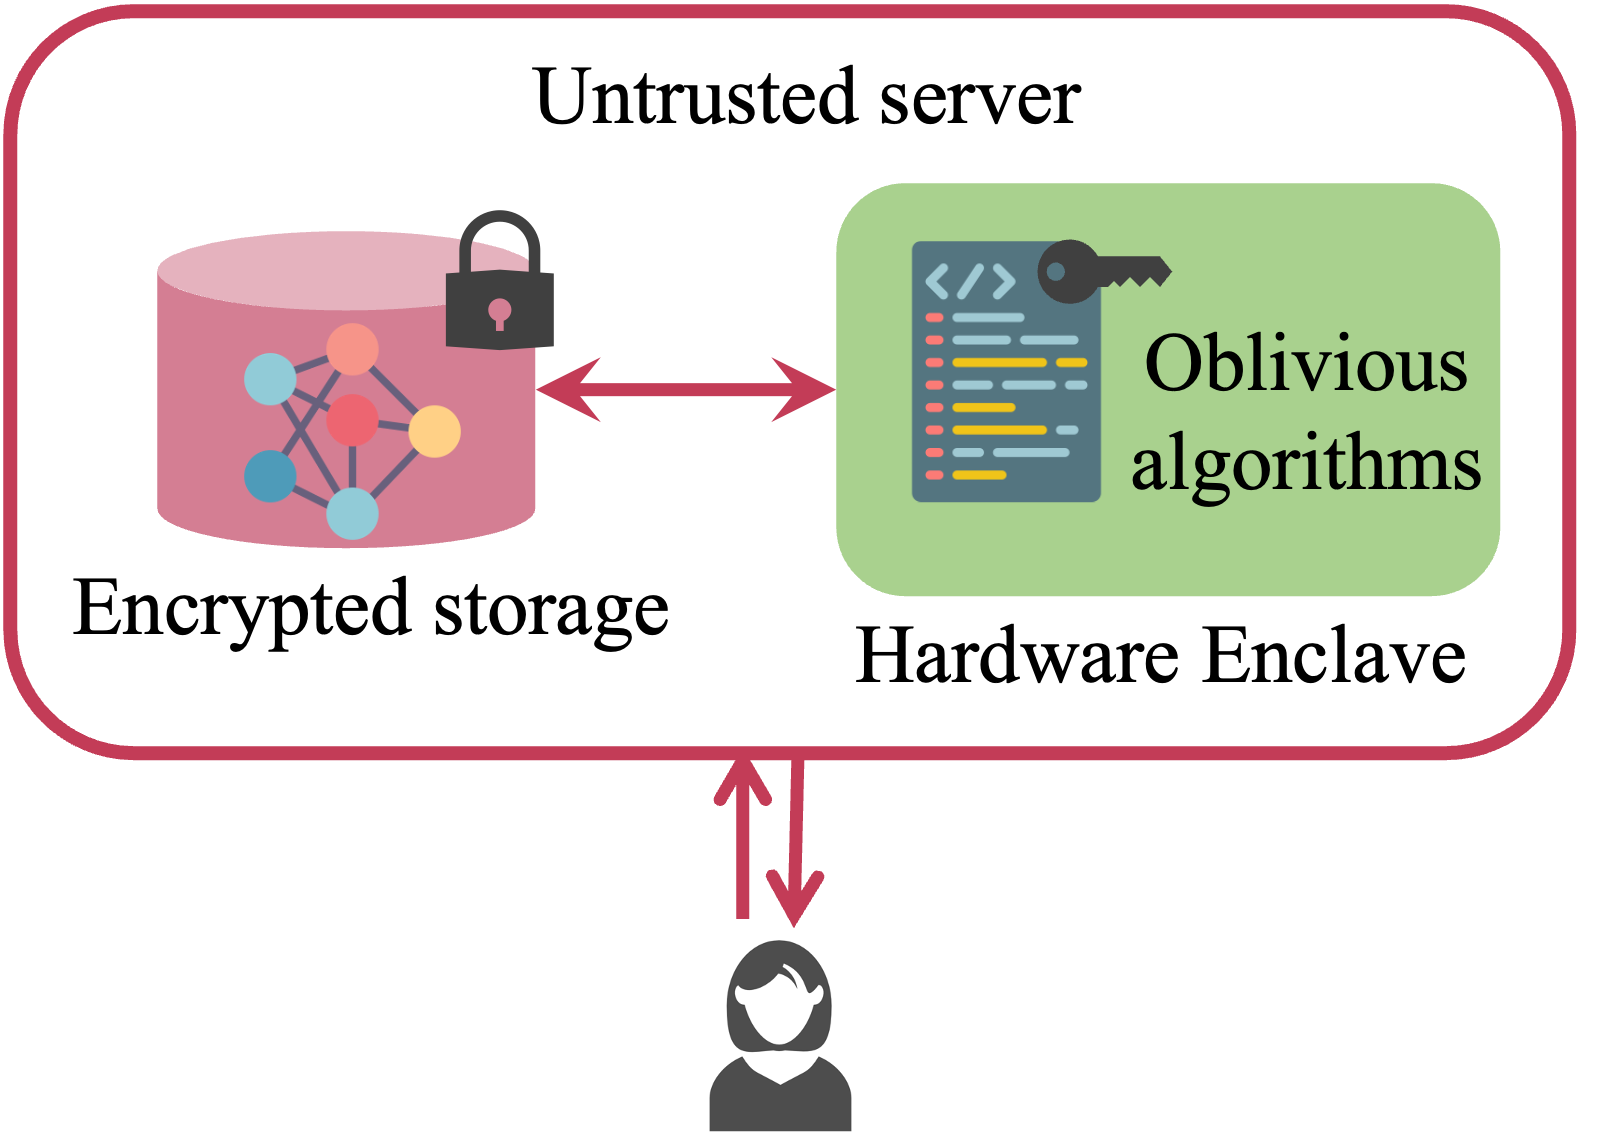
\includegraphics[scale=0.4]{figures/system-model.png}
    \vspace{-1em}
    \caption{\centering System architecture of an enclave-based oblivious graph database} 
    \label{fig:sys-model}
    \Description{}
    \vspace{-1em}
\end{figure}


We consider an architecture where an application, acting as the data owner, 
outsources its data storage and computation to a cloud provider, as 
illustrated in Figure~\ref{fig:sys-model}. The data is structured as a 
property graph, consisting of multiple types of nodes, called \textit{node 
labels}, connected by one or more types of edges, called \textit{edge 
labels}. To protect data privacy from a potentially untrusted cloud 
provider, the data owner encrypts the graph using secure encryption schemes 
such as AES before outsourcing it. Clients, considered to be trusted and 
hence have permissions to query the data, send Cypher~\cite{opencypher} queries to the 
server. An oblivious graph database program running within a hardware 
enclave processes client requests by retrieving encrypted data from persistent 
cloud storage (e.g., AWS S3 buckets) and executes oblivious query processing
algorithms.


\subsection{Threat Model}

%\noindent\textbf{\underline{Threat model}}: 
In discussing the challenges and future 
research directions for oblivious graph databases, we adopt a commonly used 
threat model in enclave-based approaches~\cite{dauterman2021snoopy, krastnikov2020efficient, mishra2018oblix, chamani2023graphos, mavrogiannakis2025obliviator}, where 
the attacker can observe the server's encrypted network traffic, manage the 
software stack outside the enclave, and monitor memory accesses both inside 
and outside the enclave at cache line granularity. However, the adversary 
cannot breach the secure processor or access its secret key. The attacker 
may leverage observable information to launch side-channel attacks, including cache attacks~\cite{brasser2017software, hahnel2017high, moghimi2017cachezoom, schwarz2017malware}, branch prediction and
paging-based attacks~\cite{lee2017inferring, van2017telling, xu2015controlled}, 
and memory bus snooping~\cite{lee2020off}. Attacks based on power 
consumption and timing analysis are considered out of scope for this model.

In protecting data from such an adversary, oblivious systems often consider 
certain information about the data to be public and do not attempt to hide 
it from the adversary. For instance, oblivious RDBMSs allow public 
knowledge of the schema, the number of tuples per table, the type of 
queries executed by clients, and the final output 
size~\cite{mavrogiannakis2025obliviator, krastnikov2020efficient, popa2011cryptdb, eskandarian2019oblidb}. Similarly, 
GraphOS~\cite{chamani2023graphos} exposes equivalent information for graph data. In the context of an oblivious property graph database, we consider 
the number of nodes and edges per label, the type of query executed by 
clients, and the final query output size as public information. However, 
any intermediate output size must remain hidden from the adversary.
% , which presents a significant challenge in the design of an oblivious graph database.

% \rjm{depending on space, you might add an example of an intermediate size for a graph query that is clearly revealing information.  And if it is in a way a relational query wouldn't leak information, that would be great.}

\subsection{Data Model}
\label{sub:data-model}
We model the property graph~\cite{robinson2015graph} data with nodes, edge
relationships, and properties, similar to plaintext graph databases.
\begin{itemize}[leftmargin=*]
    \item \textbf{Node:} Each node type, identified using a
    \textit{label}, represents an entity in the data. Within each node label, we identify discrete nodes using a unique numerical id starting from 0.
    \item \textbf{Edge relationship:} An edge relationship,
    referred to simply as edges here onward, represents a connection between nodes (either of same or different labels). Similarly to the nodes, each edge type is identified by
    an \textit{edge label}. 
    %with each edge within a label identified by a unique numerical id starting from 0. 
    Each edge connects a source node to a destination node, and the edges are uni-directional. 
    %In this model, we restrict two nodes to be connected by unique edge labels.
    \item \textbf{Property:} Each node and edge label can consist of a number of properties, storing more descriptions about the data.
\end{itemize}

\subsection{Storage Model}
\label{sub:storage-layer}

Storage models used in existing oblivious databases pose unique
challenges for efficiently storing graph data. Current oblivious databases 
either store data in key-value format~\cite{dauterman2021snoopy, mishra2018oblix} or row-wise tabular format~\cite{zheng2017opaque,eskandarian2019oblidb,mavrogiannakis2025obliviator}. GraphOS~\cite{chamani2023graphos} stores graph 
data as key-values using an oblivious AVL tree, which incurs
$O(polylogN)$ overhead to access \textit{each node or edge} in the 
graph. This becomes a performance bottleneck with a graph of 
millions of nodes and edges. While graph data
can be stored in a row-wise tabular format, as seen in 
plaintext graph databases, such a storage model is inefficient 
for graph analytics. Hence, we advocate for a model that is conducive for graph analytics:
\textit{a disk-based columnar storage}, where each node or edge 
property will be stored in a separate column file.  

\begin{figure}[t]
    \centering
    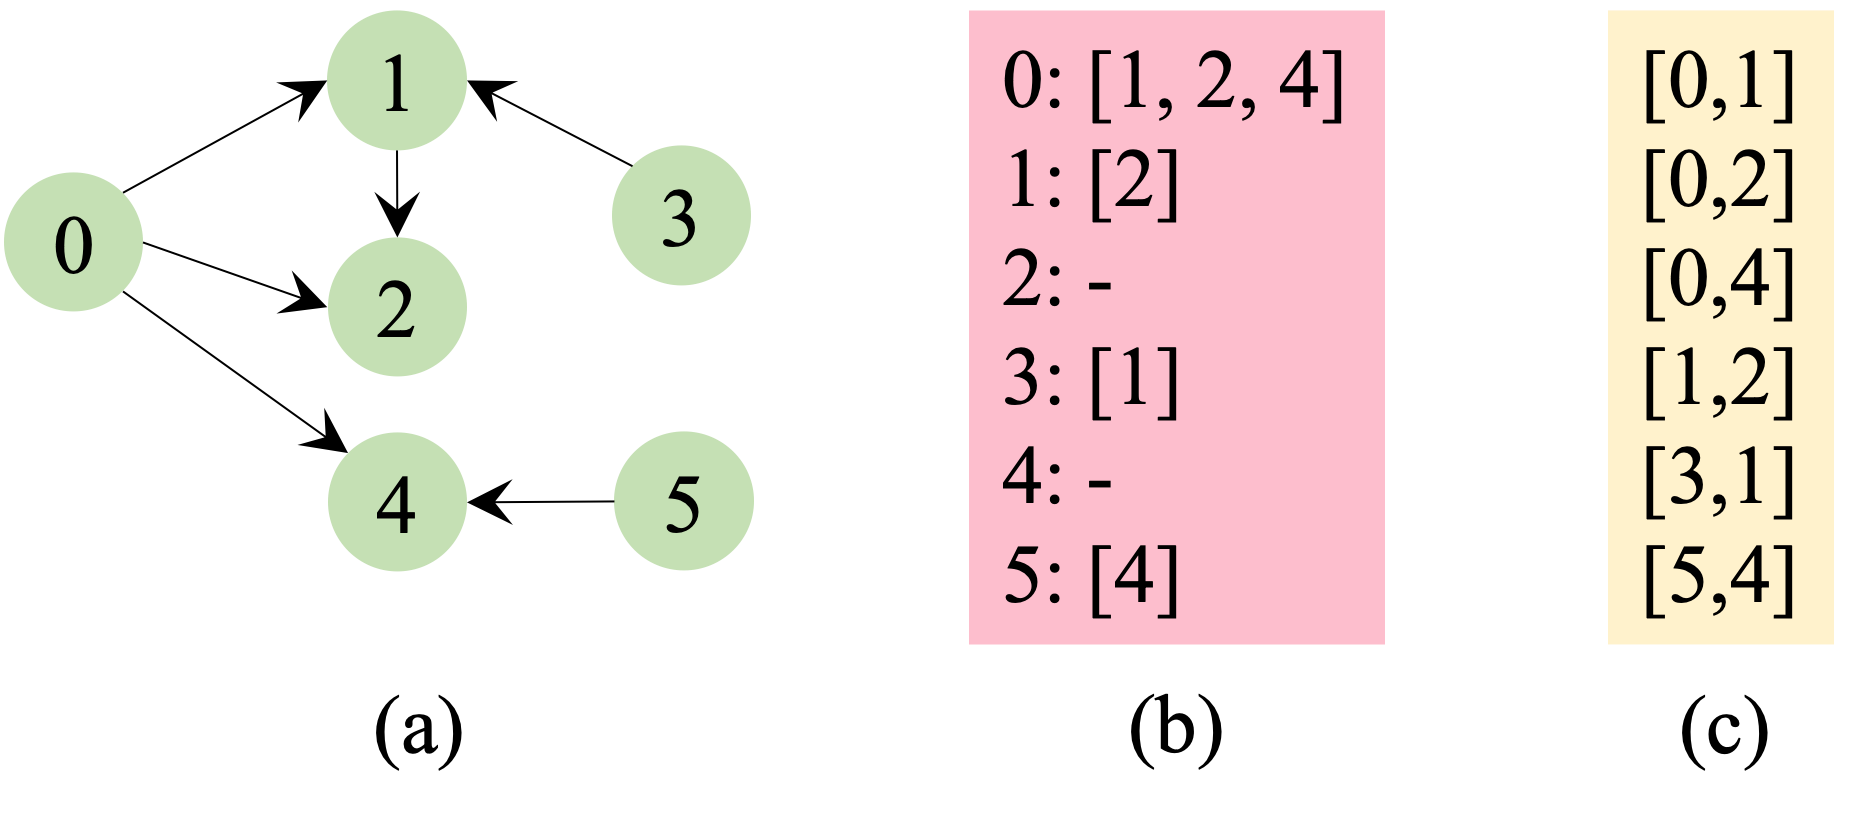
\includegraphics[scale=0.4]{figures/edge_storage.png}
    \vspace{-1em}
    \caption{\centering (a) Sample graph data. (b) Insecure edge representation. (c) Secure edge storage. } 
    \label{fig:edge-storage}
    \Description{}
    \vspace{-1em}
\end{figure}

Plaintext graph databases typically store the edges using an
adjacency list, as seen in Figure~\ref{fig:edge-storage}(b). However, this representation
is insecure because it reveals the degree of
each node, even when the ids are encrypted. Hiding this information
would require padding the adjacency list to a size of
$m\times n$, where $m$ is the number of edges and $n$ the nodes, because
in the worst case, all $m$ edges can originate from a single
node. Therefore, we propose to store the adjacency in a single
array-like format, sorted on the ids of the source nodes
as shown in Figure~\ref{fig:edge-storage}(c). This only exposes $m$, the number of edges (of
a particular label), which is considered non-sensitive. 
Additionally, similar to plaintext graph databases designs such as~\cite{janusgraph,feng2023kuzu,deutsch2019tigergraph,sun2015sqlgraph}, we recommend maintaining \textit{reverse edges}
stored in the sorted order of destination node ids (also of size $m$) to enable 
bi-directional parallel processing of graph queries. While many plaintext 
graph databases use columnar storage and forward-\&-reverse edge lists,
to our knowledge, we are the first to deviate from the key-value or tabular format in oblivious databases.


% \rjm{Has the secure storage (2(c)) proposed here been used before?  I'm wondering about novelty and if this specific representation allows reverse edges that are secure (don't reveal information).?}
% \vspace{-0.5em}
\section{Graph Query Processing}
\label{sec:graph_qp}

Having described the system architecture and the storage model, we now
discuss challenges introduced by executing typical graph database queries 
obliviously.

\vspace{-1em}
\subsection{0-hop query}
\label{sub:0-hop}

We begin by examining the simplest type of query in graph databases involving a single 
node label with one or more predicates on its properties. This section 
highlights the challenges posed by non-oblivious query processing algorithms and provides insights 
on how to morph these algorithms to ensure obliviousness. To illustrate, let's take a sample Cypher query:
\texttt{MATCH u:user WHERE u.age $>$ 30 AND u.lives\_in = `LA' RETURN u.name}.

Consider the following code that retrieves the properties relevant to the query
and tests the predicates using an if-else statement.

\noindent\hrulefill
\begin{algorithmic}[1]
        \State Assume $ages$, $lives\_in$, and $names$ are lists that store relevant properties after reading from the storage
        \State $output \gets []$
        \For {$i$ in range(0, $num\_users$)}
            \If {$ages[i] > 30$ \&\& $lives\_in[i] == ``LA"$ } 
                \State $output.append(names[i])$
            \EndIf
        \EndFor
        \State \Return $output$
\end{algorithmic}
\noindent\hrulefill

\noindent Executing the above code within an enclave reveals the node ids of users that
satisfy the predicates to an adversary who can observe memory accesses because the 
$output$ variable is accessed and modified only when the predicates are true. 
One way to execute the above functionality obliviously is to use a ternary
operator:

\noindent\hrulefill
\begin{algorithmic}[1]
        \State $output \gets []$
        \For {$i$ in range(0, $num\_users$)}
            \State \parbox[t]{\linewidth}{$res \gets (ages[i] > 30$ \&\& $lives\_in[i] == ``LA"$)?\newline \null\hspace{9mm} $names[i]$ : $``dummy"$} 
            \State $output.append(res)$
        \EndFor
        \State \Return obliviousCompact($output$)
\end{algorithmic}
\noindent\hrulefill

This code modifies the $output$ for each user, ensuring identical 
memory accesses for all node ids. The $output$ can then be 
compacted obliviously using an \textit{oblivious compaction} 
mechanism, such as~\cite{goodrich2011data, sasy2022fast}, to remove dummies before 
returning the result to the client.
Existing oblivious 
databases~\cite{eskandarian2019oblidb, zheng2017opaque, mavrogiannakis2025obliviator, krastnikov2020efficient} employ 
such strategies for processing relational queries. 

\subsection{1-hop query}

Having used the simple 0-hop query to provide intuitions on processing queries
obliviously, this section discuss challenges and future research directions
stemming from 1-hop queries. A 1-hop query spans two distinct node labels $n1$ and $n2$ (we discuss cyclic queries in~\cref{sub:cyclic})
connected by an edge $e$ of the form: $n1 - e \rightarrow n2$, with predicates on any node
or edge label.

\noindent\textit{\textbf{1. Challenges with processing 1-hop query using
existing relational operators.}} One way to process such queries is to consider the two nodes and the edge as relations and use 
oblivious binary join operators~\cite{mavrogiannakis2025obliviator,krastnikov2020efficient, eskandarian2019oblidb,zheng2017opaque}: first join $n1$ with $e$, then join the
output of that with $n2$. Because the edge relation exhibits primary-key-foreign-key relationship with both the node relations, the output of both the joins will
be $|e|$, the number of edges. 

Naively executing a sort-merge join, the most adopted join technique in oblivious settings
~\cite{zheng2017opaque, eskandarian2019oblidb, krastnikov2020efficient, mavrogiannakis2025obliviator},
reveals how many times each join key is repeated based on the pointer traversal pattern 
in the merge step. Existing solutions counter this leakage by first concatenating the two 
input tables and obliviously sorting it on the $<$join key, table id$>$ pair, which in our case, sorts a table of $|n_i| + |e|$ size. This sorted concatenated table
helps identify the join keys present in both tables and how many times each key appears in
the output based on the product of its count in each table.

Applying any of these join algorithms~\cite{zheng2017opaque, eskandarian2019oblidb, krastnikov2020efficient, mavrogiannakis2025obliviator} to process a 1-hop query requires performing two joins, each involving an oblivious sort over tables of sizes 
$|n1|+|e|$ and $|e|+|n2|$. Since oblivious sorting dominates the cost of oblivious joins with 
a complexity of $O(nlog^2n)$ for a table of size $n$, this approach incurs significant 
overhead when $|n|$ and $|e|$ scale to millions of nodes and billions of edges.
% Recall from \cref{sub:storage-layer} that graph databases store the node and edge information already in sorted
% format for better query efficiency.
% But existing oblivious join 
% operators do not take advantage of this because \textit{they all require merging the
% input tables and obliviously sorting it on the join key to identify join keys
% present in both tables}.
This raises the first research question:

\begin{tcolorbox}[colback=gray!7!white,coltitle=black,colframe=orange!50!white,title=\centering \textbf{Research question 1}]
\centering
\emph{Can we design a new oblivious binary join operator that identifies join
keys present in both tables \textbf{without} concatenating and sorting the two input tables?}
\end{tcolorbox}

\noindent\textit{\textbf{Towards a solution}}: One way to identify join keys
present in both tables is to hash the join keys of one table $T1$ and store it 
in a hash map and probe the second table $T2$ by hashing the join keys and checking if
the hashed value is present in the hash table (i.e., a hash join). This solution 
identifies join keys
present in both tables without requiring to concatenate and sort them. However, skew
in the join key distribution reveals sensitive information to an adversary:
if $T1$ has many repeated join keys, this will create hash collisions, revealing
the skew in the data. Alternatively, repeated join keys in $T2$ will repeatedly
probe the same hash bucket, also revealing the skew in the
data. Thus, the oblivious join scheme should protect against such leakages by
considering potential solutions such as key de-duplication and oblivious aggregation operations. 
% Such a join operator will be applicable to many applications where
% the two inputs to the operator come pre-sorted.

\vspace{0.7em}
\noindent\textit{\textbf{2. Challenges with relying on relational operators.}} 
Even with a new efficient oblivious binary join protocol that removes the need
to sort a large concatenated table, executing a 1-hop query using relational
operators incurs high latency because the two joins must be executed \textit{sequentially}.
% Additionally, the most efficient oblivious binary join~\cite{mavrogiannakis2025obliviator},
% which is a sort-merge join algorithm, requires an intermediary sort of the size of the 
% output, which in our case is
% $|e|$. This sort is necessary to align the join keys of the two tables before the 
% final merge phase~\cite{krastnikov2020efficient,mavrogiannakis2025obliviator}.
% Hence, with two joins, this approach sorts two intermediary tables of size $|e|$,
% \textit{sequentially}.
This raises the next research question:

\begin{tcolorbox}[colback=gray!7!white,coltitle=black,colframe=orange!50!white,title=\centering \textbf{Research question 2}]
\centering
\emph{Can we design a custom \textbf{parallelizable} oblivious query processing algorithm to serve 1-hop queries without relying on oblivious binary joins?}
\end{tcolorbox}

\noindent\textit{\textbf{Towards a solution}}: In designing a new oblivious algorithm
to avoid the above sequential processing, we look at plaintext graph databases
that process such queries from \textit{two directions} in parallel: $n1\rightarrow e$
and $e \rightarrow n2$. At a high level, find all nodes ids
of $n1$ that act as the source of an edge with id $e_i$, and node ids of $n2$ that
is the destination of an edge $e_j$. This gives us two lists of edge ids; the 
intersection of these ids is the output of the query (note that we can propagate node
or edge properties along the way). However, naively executing this approach may leak 
sensitive information such as
% \rjm{I think you want to say "the number of nodes with an edge of type e", right?  Or do you me the list of nodes themselves are leaked?}  
the number of unique nodes from $n1$ and $n2$ with an edge label $e$ and the edges in the final output. Hence, this creates the need for custom 1-hop operator 
that traverses the forward and reverse edge lists in parallel to compute the output 
without revealing any sensitive information.

\vspace{-0.7em}
\subsection{2-hop queries and beyond}

Next, we discuss the challenges introduced by multi-hop queries
spanning three or more nodes, connected by two or more
edges.

\noindent\textit{\textbf{Challenges with intermediary result size leakages}}. For
1-hop queries, whether executed using oblivious relational operators or custom query 
processing algorithms, the output or intermediary sizes are bounded by $|e|$, which
is considered non-sensitive. However, expanding the system to support
multi-hop queries introduces the challenge of hiding intermediary result sizes.
Naively addressing this by applying worst-case padding — pad an intermediate result to its worse possible size — significantly degrades system performance. 
For example,
for a 2-hop query spanning edges $e_1$ and $e_2$, worst-case padded intermediary table
will be of size $|e_1| \times |e_2|$.


\begin{tcolorbox}[colback=gray!7!white,coltitle=black,colframe=orange!50!white,title=\centering \textbf{Research question 3}]
\centering
\emph{Can we develop more \textbf{efficient} mechanisms to hide or obfuscate intermediary result sizes without resorting to worst-case padding?}
\end{tcolorbox}

\noindent\textit{\textbf{Towards a solution}}: Computing the size of any table is 
equivalent to computing the COUNT aggregate function on a table. Differential privacy (DP) \cite{DworkRoth2014} is an ideal technique for hiding the exact results of an aggregate query. Shrinkwrap \cite{Bater2018} was
the seminal work that applied DP to hide or obfuscate intermediary result sizes of
a SQL query consisting of multiple operators. However, it considered a privacy budget
$\epsilon$ allocated to each query executed by the system. Thus, the \textit{global 
privacy budget} increases significantly per executed query, potentially revealing more
than anticipated amount of sensitive information. Alternatively, solutions such as 
Turbo \cite{Kostopoulou2023} and cacheDP \cite{Mazmudar2022} cache the DP-derived noise for queries and reuse them when queries
are repeated to reduce the consumption of the global privacy budget for each query. 
However, the proposed techniques only apply for \textit{linear queries} where queries 
span a single table. As discussed so far, queries in graph databases cover many nodes
and edges, and the process of joining them amplifies query sensitivity, thereby increasing 
the required noise budget. Hence, this challenge presents new research opportunities in 
caching DP-noise for complex queries that span multiple entities or tables.

\vspace{-0.7em}
\subsection{Cyclic queries}
\label{sub:cyclic}

A common query pattern observed in property graph databases are cyclic
queries of the form $n1 - e1 - n2 \- \cdots e_i - n1$.

\noindent\textbf{\textit{Challenges with cyclic queries}}. While cyclic queries can be 
executed with a 
series of binary joins, such an approach often generates 
exponentially large intermediate results~\cite{ngo2014skew}, significantly 
degrading performance in oblivious settings due to their inherent computational overhead.
For instance, consider the query: "users who are friends and have purchased the same product." This forms a cyclic pattern: (u1:User) - [:FRIEND] → (u2:User) - [:PURCHASE] → (:Product) ← [:PURCHASE] - (u1:User). A 
binary join approach might first compute all User-Friend pairs (potentially $O(U^2)$ for $U$ users), then join with Purchases to find shared products. For example, with 1,000 users, each having 100 friends and 10 purchases, the User-Friend join alone produces 100,000 pairs, which, when joined with Purchases, results in 1,000,000 intermediate tuples—most of which are discarded later.

\begin{tcolorbox}[colback=gray!7!white,coltitle=black,colframe=orange!50!white,title=\centering \textbf{Research question 4}]
\centering
\emph{Can we device oblivious join algorithms for complex cyclic joins that are
asymptotically \textbf{faster} than a sequence of binary joins?}
\end{tcolorbox}

\noindent\textit{\textbf{Towards a solution}}:
Worst case optimal joins (WCOJ)~\cite{ngo2018worst} handle cyclic queries more efficiently by evaluating multi-way intersections column-at-a-time rather than table-at-a-time, achieving the theoretical worst case output size defined by the AGM bound~\cite{atserias2008size} (e.g., $n^{3/2}$ for a cycle of 3). In the example above, processing the query using WCOJ 
simultaneously tracks the user-friend relation and the intersecting purchases, which prunes non-matching paths early. While a few oblivious acyclic
multi-way joins have been proposed in the past~\cite{arasu2013oblivious, chu2021differentially}, Hu and Wu~\cite{hu2025optimal} recently
proposed the first oblivious WCOJ construction. However, their construction pads the output to a query-dependent worst-case
size (i.e., $O(n^f)$ where $f$ indicates fractional edge cover), which we believe
can be further reduced. Additionally, all the above discussed papers~\cite{arasu2013oblivious, chu2021differentially,hu2025optimal} are theoretical in nature with no implementation to show empirical results. Hence, developing practical oblivious
WCOJs for a secure property graph database remains an open area of research. 
% Property graphs benefit from WCOJ's ability to handle cyclic many-to-many relationships, it is common in recommendation systems (e.g. friends who liked the same items) or fraud detection (e.g. cycles of transactions).  


%==============================================================================
\section{Evaluation}
\label{sec:evaluation}
%==============================================================================

We evaluate \system against two state-of-the-art oblivious join baselines,
answering three questions:
\begin{enumerate}[leftmargin=*]
    \item How does \system compare against existing oblivious join approaches
    on multi-hop graph queries, across real and synthetic graphs of up to
    180M edges? (\cref{sec:evaluation:cross})
    \item Does \system generalize beyond chain queries to other join
    topologies such as fan-in, fan-out, and tree patterns?
    (\cref{sec:evaluation:shapes})
    \item Is \system's cost truly independent of the size of the unfiltered
    intermediate result, as promised by in-place filtering?
    (\cref{sec:evaluation:density})
\end{enumerate}

%------------------------------------------------------------------------------
\subsection{Experimental Setup}
\label{sec:evaluation:setup}
%------------------------------------------------------------------------------

All experiments run inside an Intel TDX guest VM on a recent Intel Xeon host,
with X vCPUs (X physical cores, 2-way SMT), 471 GB of RAM, and Ubuntu
24.04 (Linux 6.8). \sujaya{@Bish: State how much was used, not necessarily how much the machine supports.} By default, we run \system and its baseline with 64 threads.

\noindent\textbf{Baselines.}
We compare \system with:
\begin{itemize}[leftmargin=*]
    \item \textit{Full MWJ}: A system executing a graph query as an oblivious multi-way join (MWJ) using
    \wei \cite{ruidi2025oblivious} executed over the full, non-decomposed
    query, with predicate filtering applied after the join.
    \item \textit{Obliviator chained}: The state-of-the-art oblivious
    join scheme of Obliviator~\cite{mavrogiannakis2025obliviator}, applied
    hop-by-hop: each hop is an oblivious two-table join whose output is
    re-keyed and fed to the next hop.
    % We note that chaining two or more hops \textit{reveals
    % multiple intermediary result sizes}, making this baseline strictly weaker in
    % security for hops $>$1.

\end{itemize}

\begin{table}[t]
\centering
\caption{Leakage profile of the compared systems: which result sizes each
system reveals to an adversary observing memory. All systems reveal the
(public) input table sizes.}
\label{tab:leakage}
\begin{tabular}{lccc}
\toprule
 & \textbf{Hop-to-hop} & \textbf{Unfiltered} & \textbf{Filtered} \\
\textbf{System} & \textbf{intermediates} & \textbf{join output} & \textbf{output} \\
\midrule
Obliviator & revealed & revealed & revealed \\
Full MWJ & \textbf{hidden} & revealed & revealed \\
\system & \textbf{hidden} & \textbf{hidden} & revealed \\
\bottomrule
\end{tabular}
\end{table}

The three systems provide different security guarantees, summarized in
\Cref{tab:leakage}. Obliviator's chained execution materializes every
hop-to-hop intermediate join size at its true cardinality, which can be
a sensitive signal about graph structure. Full MWJ hides all intermediates inside the multi-way join, but must
materialize the \emph{unfiltered} join output before filtering, revealing
its size. \system reveals only the final \emph{filtered} output size as the
unfiltered intermediate is never materialized. \system therefore has
the strictest leakage profile of the three; where we nevertheless include
the leakier baselines, we are giving them the benefit of the doubt.

\smallskip
\noindent\textbf{Datasets.}
\Cref{tab:datasets} lists the six graph datasets we use in the evaluations.
\emph{Banking} is a synthetic
financial transaction graph produced by a seeded generator (1M accounts,
5M transactions, near-uniform degrees). The \emph{IBM AML} HI-Small, HI-Medium,
and HI-Large graphs are anti-money-laundering transaction networks from
IBM's AMLworld~\cite{altman2023realistic}; their degree
distributions are heavy-tailed, with hub accounts that participate in a
large fraction of transactions. \emph{LDBC SNB} is the person--knows--person
friendship graph of the LDBC Social Network Benchmark (Interactive
workload, scale factor 30)~\cite{erling2015ldbc}: a dense small-world
social network whose undirected friendships we mirror into directed edges,
giving an average degree of 73, an order of magnitude denser than the other
graphs. \emph{SNAP cit-Patents} is the US patent
citation network~\cite{snapnets}, a sparse citation DAG (average
out-degree 4.4).
% Besides node and edge counts, the table
% reports the number of \emph{unfiltered 2-hop paths},
% $\sum_a \mathit{in}(a)\cdot \mathit{out}(a)$ --- the size of the intermediate
% that a join-then-filter system must process for a 2-hop query. Skew
% decouples this quantity from edge count: Banking and HI-Small have the same
% number of edges, but HI-Small has $15\times$ more 2-hop paths; HI-Medium has
% $6\times$ more edges than cit-Patents but $146\times$ more paths.

\begin{table}[t]
\centering
\begin{tabular}{lrrr}
\toprule
\textbf{Dataset} & \textbf{Nodes} & \textbf{Edges} \\
\midrule
Banking (synthetic) & 1.0M & 5.0M \\
IBM AML HI-Small & 515K & 5.1M \\
LDBC SNB (SF30) & 165K & 12.0M \\
SNAP cit-Patents & 3.8M & 16.5M \\
IBM AML HI-Medium & 2.1M & 31.9M \\
IBM AML HI-Large & 2.1M & 179.7M \\
\bottomrule
\end{tabular}
\caption{Datasets.}
\label{tab:datasets}
\end{table}

\smallskip
\noindent\textbf{Queries.} We evaluate all three systems on multi-hop
queries, going up to X hops. Further, we evaluate \system on various join
patterns (chains, fan-in, fan-out, tree). When querying the synthetic
dataset, we leverage the query from \cref{sec:overview} mimicking a
fraud-detection query: starting from a flagged entity, follow $k$
node--edge--node hops and return the matching paths.
\system leverage the query decomposer to breakdown a query into on-hop
instances and construct a final residual query; baselines execute
the original query. The exact queries for each experiment can be
found in [].

\smallskip
\noindent\textbf{Reported timing.}
For each experiment, we report the time it took to execute a query.
We give each experiment a budget of one hour and the
full machine, and report runs exceeding the budget as timeouts (T/O) and
runs exhausting the 471 GB of memory as out-of-memory (OOM). Because many
experiments run for tens of minutes to hours, we report a single measured run per
cell, which we precede with a discarded warm-up run; repeated executions of
the faster experiments vary by at most $2\%$.
% We validate the output of every
% completing run against a plaintext SQLite baseline, and we additionally
% check output cardinalities against analytically computed ground truth.

%------------------------------------------------------------------------------
\subsection{Comparison on Real-world Datasets}
\label{sec:evaluation:cross}
%------------------------------------------------------------------------------

\begin{figure*}[t]
\centering
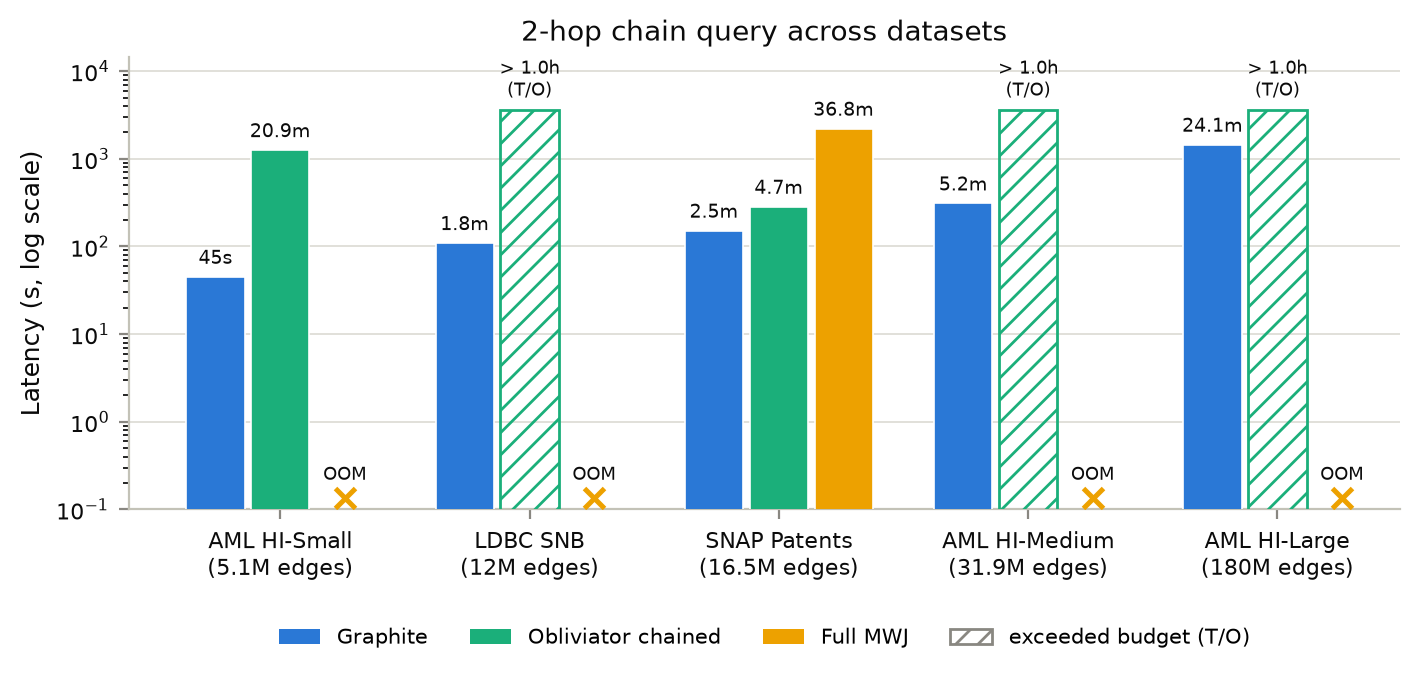
\includegraphics[width=0.65\textwidth]{figures/e3_cross_dataset.png}
\caption{A 2-hop query across five datasets (log-scale latency).}
\label{fig:cross_dataset}
\end{figure*}

\Cref{fig:cross_dataset} shows the result of comparing the three systems on
the five non-synthetic datasets, evaluated on a 2-hop query.

\system completes on every dataset, whereas each baseline completes on only
two of the five. Obliviator finishes HI-Small and cit-Patents but times out
on LDBC SNB (12M edges), HI-Medium, and HI-Large; Full MWJ completes only
cit-Patents and goes out-of-memory on the other four. On the datasets where a
baseline does complete, \system is $1.9$--$28\times$ faster than Obliviator
(which reveals intermediate sizes) and $14\times$ faster than Full MWJ on
the patent dataset. We note several counter-intuitive results: Obliviator takes
less time on the 16.5M-edge patent graph than on the 5.1M-edge HI-Small
graph; Full MWJ goes out-of-memory on the smaller HI-Small graph while
completing on the larger patent graph; and both baselines fail on the
12M-edge LDBC SNB graph while completing on the patent graph, which has
$1.4\times$ more edges. All of these occur because baseline cost is governed
by the size of the unfiltered intermediate join rather than the edge count.
The patent graph is sparse, so its 2-hop join produces 82.2M unfiltered
rows; HI-Small's hub accounts inflate its intermediate to 355.1M rows
despite a third of the edges; and SNB's uniformly high degree inflates it to
3.3B rows --- $40\times$ the patent graph's, from fewer edges. Notably, SNB
shows that this blowup does not require skewed hubs: on a dense graph,
\emph{every} node's in--out product is large. We study this effect in
detail in \cref{sec:evaluation:density}.

This experiment also highlights \system's scalability: as the graph grows
from the 16.5M-edge patent dataset to the 179.7M-edge AML HI-Large dataset,
\system smoothly handles the increase and completes the 2-hop query in
24.1 minutes, whereas Full MWJ runs out of memory. Despite revealing intermediary results,
even Obliviator fails on a 2-hop query on large inputs --- and, on the dense
SNB graph, already on a moderately sized one.




% These observations set up the remaining two experiments. Obliviator's
% chained kernel is a linear pipeline whose efficiency depends on
% revealing per-hop sizes; it supports only chain-shaped queries, and
% extending it to other topologies would require new kernels and yet more
% leakage. We therefore exclude it from the topology experiment and compare
% against the fully hiding Full MWJ (\cref{sec:evaluation:shapes}). Second,
% the correlation between baseline cost and intermediate size suggests that
% the unfiltered intermediate --- not the graph itself --- is what baselines
% pay for; \cref{sec:evaluation:density} isolates exactly this variable.

\subsection{Impact of Graph Density}
\label{sec:evaluation:density}
%------------------------------------------------------------------------------
\begin{figure}[t]
\centering
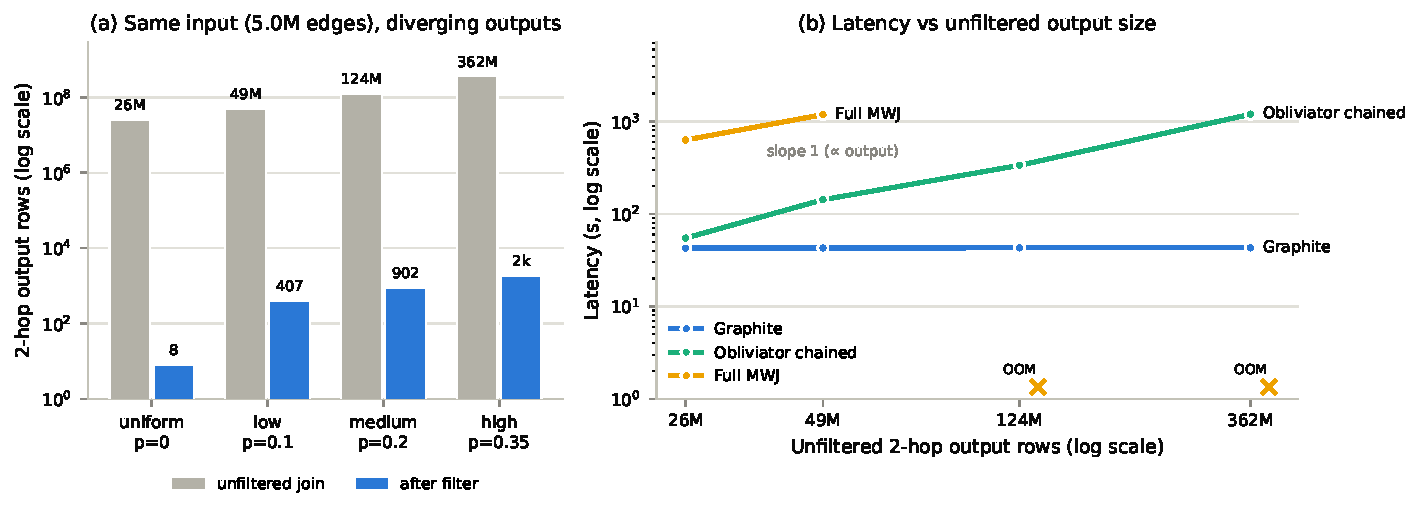
\includegraphics[width=\linewidth]{figures/e5_density_5M.png}
\caption{Impact of density on fixed-size inputs (1M nodes, 5M
edges). \system's latency remains roughly constant despite the unfiltered join
result size increasing from 29.1M to 362.1M rows due to increase in graph density,
which affects the baselines.}
\label{fig:density}
\end{figure}

The real-world dataset experiment hinted that graph density plays a vital
role in baseline performance, but it varied graph size, output size, and
density simultaneously. To isolate the effect of density alone, we use the
synthetic banking dataset and hold both the input size (1M accounts, 5M
transactions) and the final output size (under 2000 tuples) fixed. We
generate four variants that differ only in how edges concentrate on a
small set of hub accounts (hub fraction $p \in \{0, 0.1, 0.2, 0.35\}$).
Raising $p$ increases graph density directly, inflating the unfiltered
2-hop join from $26.1$M to $362.1$M rows as the graph becomes more
dense, producing a $13.9\times$ increase in join output size.

\Cref{fig:density} shows the results. Both baselines slow down as density
increases: Full MWJ's latency grows from 10.5 minutes at 26M unfiltered
rows to 19.7 minutes at 49M, then runs out of memory beyond 124M rows.
Obliviator degrades from 55 seconds to 19.9 minutes, a $21.8\times$
slowdown. \system, by contrast, holds latency flat at $42.7$--$43.1$s
across the experiment, despite the unfiltered
intermediate growing by $13.9\times$.

This experiment highlights two points. First, unlike the baselines, \system is
agnostic to density-driven blow-up in intermediate join size --- a
property especially valuable for property graph databases, where graph
structure routinely produces large intermediates even when the filtered
output stays small. Second, it provides empirical evidence for \system's
obliviousness guarantee: adversary-observable behavior should depend only
on public information, and since both input and output sizes are held
fixed here, \system's observable runtime remains unchanged too. The baselines, by
contrast, leak the graph's density through their running time alone.


%------------------------------------------------------------------------------
\subsection{Generality Across Query Topologies}
\label{sec:evaluation:shapes}
%------------------------------------------------------------------------------

Chain queries are only one traversal pattern. Analysts also ask
\emph{fan-in} queries (find $m$ distinct transactions converging on a
flagged account, a smurfing pattern), \emph{fan-out} queries ($m$
transactions leaving a flagged account, a dispersal pattern), and \emph{tree}
queries combining both. \system handles these topologies without
modification: the query decomposer turns \emph{every} edge of the join
graph into an independent \onehop operator regardless of shape, and only
the residual join structure changes. We run 2/3/4-hop chains plus a
fan-in, fan-out, and tree query, each with 4 edges, on AML HI-Small,
comparing \system against the baselines. We omit Obliviator on non-chain
queries because extending it beyond chains requires a non-trivial wrapper.

\begin{table*}[t]
\centering
\label{tab:shapes}
\begin{tabular}{lrrrrrr}
\toprule
\textbf{Query} & \textbf{Edges} & {\textbf{Unfiltered size}} & \textbf{Filtered size} & \textbf{\system} & \textbf{Full MWJ} & \textbf{Obliviator} \\
\midrule
1-hop & 1 & 5.1M & & & &\\
2-hop  & 2 & 355M & & 43\,s & OOM &\\
3-hop & 3 & 6.6B & & 84\,s & OOM &\\
4-hop & 4 & 134B & & 137\,s & OOM &\\
fan-in & 4 & 1.7T & 8M & 254\,s & OOM &\\
fan-out & 4 & $9.2{\times}10^{20}$ & 9.7M & 281\,s & OOM &\\
tree & 4 & $6.9{\times}10^{14}$ & 4.2M & 194\,s & OOM &\\
\bottomrule
\end{tabular}
\caption{Query topologies on AML HI-Small. ``Unfiltered rows'' is the
exact size of the intermediate a join-then-filter system must materialize.
Full MWJ exhausts the machine's RAM on every topology; Obliviator....}
\end{table*}

% \Cref{tab:shapes} shows the results. \system completes every topology in
% under five minutes, including the 4-edge star and tree patterns whose
% final outputs has millions of rows. Latency across the 4-edged queries varies
% only with the number of residual joins and the output size, not with the shape
% itself --- fan-in, fan-out, and
% tree each take within $1.4$--$2.1\times$ the latency of 4-edged
% chain. Full MWJ, by contrast, fails with out-of-memory on every topology,
% due to large unfiltered sizes.
% The ``unfiltered rows'' column explains why, and
% shows that this is not a memory-budget artifact: star and tree topologies
% compound hub degrees multiplicatively (fan-in over a node of in-degree $d$
% contributes $d^4$ rows), driving the unfiltered intermediate to $10^{12}$-$10^{20}$
% rows; the fan-out intermediate alone would occupy roughly
% $10^{23}$ bytes. Join-then-filter is therefore not merely slow on these topologies,
% it is infeasible at any practical scale.
% Shrinking the graph does not help, since
% even a 100$\times$ smaller banking graph (50K edges) still yields a
% $1.7{\times}10^{16}$-row fan-out intermediate. \system is unaffected by
% this blowup because it does not materialize the intermediate join, and its
% star and tree queries run in the same few minutes as the equally sized
% chain.

As shown in the last experiment, the latency of the baselines depends on unfiltered
intermediate rather than the graph's edge count or query's output size. Non-chain
topologies push this further: branching causes hub degrees to
\emph{compound multiplicatively} rather than accumulate additively along a
single path. A fan-in over a node of in-degree $d$ contributes $d^4$ rows
to the unfiltered join, versus a linear contribution for a chain of the
same length. This drives the unfiltered intermediate to $10^{12}$--$10^{20}$
rows for our 4-edge fan-in, fan-out, and tree queries --- the fan-out
intermediate alone would occupy roughly $10^{23}$ bytes, twelve orders of
magnitude beyond our 471GB RAM. The effect is structural, not an
artifact of graph size: even a 100$\times$ smaller banking graph (50K
edges) still yields a $1.7{\times}10^{16}$-row fan-out intermediate.
Join-then-filter is therefore not merely slow on these topologies; it is
infeasible at any practical scale, which is why Full MWJ goes out-of-memory
on every row of \cref{tab:shapes}.

\system is unaffected by this blowup, since it never materializes the
intermediate: \cref{tab:shapes} shows every topology completing in under
five minutes, including the fan-in, fan-out, and tree queries, whose
filtered outputs still run to millions of rows (8.0M, 9.7M, and 4.2M
respectively). Latency instead tracks the residual join structure and the
output size --- fan-in, fan-out, and tree each take within
$1.4$--$2.1\times$ the latency of the 4-hop chain, despite their unfiltered
sizes differing by up to eight orders of magnitude.

%------------------------------------------------------------------------------
\paragraph{Summary.}
Across all three experiments, the pattern is the same: the cost of prior
oblivious join approaches is governed by the size of intermediates they
materialize --- per-hop results for Obliviator, the unfiltered join for
Full MWJ --- and real graph workloads make those intermediates explode.
\system's costs are governed by the input size and the filtered output
size alone, which is why it completes every dataset, every topology, and
every density level in this evaluation, while leaking strictly less.

%\vspace{-0.7em}
\section{Conclusion}

Oblivious query processing for property graph databases remains an open challenge, with 
existing solutions either lacking support for general-purpose property graph queries or 
incurring significant performance overhead when modeling graphs within a relational 
framework. In this paper, we discuss the design space for an oblivious property graph 
database and highlight key research directions in storage models, query execution 
algorithms, and techniques for obfuscating sensitive intermediate results. Advancing 
these techniques will enable secure graph analytics, which is critical for privacy-sensitive domains domains such as finance and health care.



% \section*{Acknowledgements}
% We acknowledge the support of the Canada
% Excellence Research Chairs (CERC) program. Nous remercions le Chaires d’excellence en recherche du Canada (CERC)
% de son soutien. This project was made possible in-part through the support of the National Cybersecurity
% Consortium and the Government of Canada (CSIN). We also acknowledge NSERC for grant RGPIN-2023-03448.
\bibliographystyle{plain}
\bibliography{references}
\end{document}
\endinput
%%
%% End of file `sample-sigconf.tex'.
